

%*** General probabilistic notation ***

\newcommand{\expv}{\mathbf{E}} % EXP. VALUE
\newcommand{\discProbDist}{f} % Discrete prob distribution
\newcommand{\sampleSpace}{S} % Generic sample space
\newcommand{\sigmaAlg}{\mathcal{F}} % Generic sigma-algebra
\newcommand{\probm}{\mathbb{P}} % Generic probability measure, also prob. measure operator
\newcommand{\rvar}{X} % Generic random variable
%\newcommand{\dist}{\mathit{Dist}}

%*** MDP notation ***

\newcommand{\actions}{A} % The set of actions.
\newcommand{\colouring}{c} % the colouring function
\newcommand{\probTranFunc}{\Delta} % Transition function of an MDP
\newcommand{\edges}{E} % Set of edges in an MDP.
\newcommand{\colours}{C} % The set of colours in an MDP.
\newcommand{\mdp}{\mathcal{M}} % A generic MDP. 
\newcommand{\vinit}{v_0} % An initial vertex in an MDP.
\newcommand{\cylProb}{p} % Function assigning probabilities to cylinder sets in 
%the measure construction.
\newcommand{\emptyPlay}{\epsilon} %empty play
\newcommand{\objective}{\Omega} % Qualitative objective
\newcommand{\genColour}{\textsc{c}} % Generic colour
\newcommand{\quantObj}{f} % Generic quantitative objective
\newcommand{\indicator}[1]{\mathbf{1}_{#1}} % In.d RV
\newcommand{\eps}{\varepsilon} % Numerical epsilon
\newcommand{\maxc}{W} % Maximal abs. value of a colour

\newcommand{\winPos}{W_{>0}}
\newcommand{\winAS}{W_{=1}}
\newcommand{\cylinder}{\mathit{Cyl}}

\newcommand{\PrePos}{\text{Pre}_{>0}}
\newcommand{\PreAS}{\text{Pre}_{=1}}

\newcommand{\PreOPPos}{\mathcal{P}_{>0}}
\newcommand{\OPAS}{\mathcal{P}_{=1}}

\newcommand{\safeOP}{\mathit{Safe_{=1}}}
\newcommand{\closed}{\mathit{Cl}}

\newcommand{\reachOP}{\mathcal{V}}
\newcommand{\discOP}{\mathcal{D}}
\newcommand{\valsigma}{\vec{x}^{\sigma}}

\newcommand{\lp}{\mathcal{L}}
\newcommand{\lpdisc}{\lp_{\mathit{disc}}}
\newcommand{\lpmp}{\lp_{\mathit{mp}}}
\newcommand{\lpsol}[1]{\bar{#1}}
\newcommand{\lpmpdual}{\lpmp^{\mathit{dual}}}

\newcommand{\actevent}[3]{\actions^{#1}_{#2,#3}} % Returns #1-th action on the run 

\newcommand{\MeanPayoffSup}{\MeanPayoff^{+}}
\newcommand{\MeanPayoffInf}{\MeanPayoff^{-}}

\newcommand{\mcprob}{M}
\newcommand{\invdist}{\vec{z}}

\newcommand{\hittime}{T}



\Cref{1-sec:intro} answers natural questions such as: what is the book about, at whom it is aimed, and how to read it.
\Cref{1-sec:simple} defines a first model of games, which is the common denominator of (almost all) models studied in this book.

We introduce the computational models that we use in \cref{1-sec:computation} and briefly define linear programming.
In \cref{1-sec:conditions} we list the main objectives appearing in all chapters.
A few notions will be useful throughout the book: they are developed in this chapter.
We start with the notion of automata, discussed in \cref{1-sec:automata}, and then memory for strategies, in \cref{1-sec:memory}.
We then show how automata and memory structures can be used to construct reductions between games in \cref{1-sec:reductions}.
We introduce in \cref{1-sec:subgames} the notions of subgames and traps.

The notion of fixed point algorithms is central to the study of games.
We first recall the main two methods for proving the existence and computing fixed points in \cref{1-sec:fixed_points}.
We then give an overview of two prominent families of fixed point algorithms for games:
value iteration algorithms in \cref{1-sec:value_iteration} and strategy improvement algorithms in \cref{1-sec:strategy_improvement}.

\section{What is this book about?}
\label{1-sec:intro}
This chapter considers quantitative objectives defined using payoffs. 
Adding quantities can serve two goals:
the first is for refining qualitative objectives by quantifying how well, how fast, or at what cost a qualitative objective is satisfied,
and the second is to define richer specifications and preferences over outcomes.
%This chapter considers quantitative games. To model quantitative
%objectives, the set of colours on edges is $\R$. The goal of adding
%quantities is to help choosing among winning strategies that arise in
%classical games. We may thus use quantities in order to refine
%qualitative objectives, i.e.~to quantify how well / how fast / how
%costly a qualitative objective is satisfied. Quantitative objectives
%may also be used to design richer specifications that are not
%$\omega$-regular (like mean payoff for instance) or other quantitative
%specifications.
\begin{itemize}
	\item We start in~\cref{4-sec:qualitative} by studying extensions of the classical qualitative objectives. Among two strategies in a reachability game that guarantee to reach a target in ten steps or in a billion steps, we would certainly prefer the first one from a pragmatic point of view.

	\item We study \emph{mean payoff games} in~\cref{4-sec:mean_payoff}. 
	We present two algorithms for solving them, the first based on \emph{strategy improvement} and the second on a \emph{value iteration} for the related class of energy games.
	Along the way we show that parity games reduce to mean payoff games.
%	An algorithm for solving mean payoff games induces an algorithm for computing the value function using binary search.

	\item We study \emph{discounted payoff games} in~\cref{4-sec:discounted_payoff}.
	We construct a strategy improvement algorithm for computing the value function.
	We also show that mean payoff games reduce to discounted payoff games, so the previous algorithm yields an algorithm for computing the value function of a mean payoff game.

	\item We study \emph{shortest path games} in~\cref{4-sec:shortest_path}.
	They extend reachability games by requiring that Eve reaches her target with minimal cost, 
	which if the weights are all equal means \emph{as soon as possible}.
	
	\item We study \emph{total payoff games} in~\cref{4-sec:total_payoff}.
\end{itemize}
%\begin{itemize}
%\item We start in~\Cref{4-sec:shortest_path} by studying extensions of the
%  classical qualitative objectives for arenas with real numbers as set
%  of colours. Among two strategies in a reachability game that
%  guarantee to reach a winning vertex in ten steps or in a billion
%  steps, we would certainly prefer the first one in a pragmatic point
%  of view. Therefore, reachability games will turn into
%  \emph{shortest-path games} where a player wants to reach a winning
%  vertex \emph{as soon as possible}.
%\item A way to solve shortest-path games in full generality is to use
%  the famous \emph{mean-payoff games}, that have their own practical
%  motivation. We introduce and study them in~\Cref{4-sec:mean_payoff}. We solve
%  them with two algorithms, based on \emph{strategy improvement} and
%  \emph{value iteration}. We can then use a binary search algorithm to
%  compute the value of each player.
%\item Another very natural payoff consists in discounting the future,
%  to make the near-future more important. We define and solve
%  \emph{discounted-payoff games} in~\Cref{4-sec:discounted_payoff}. We obtain as a
%  corollary a direct (without the need of binary search for the value)
%  algorithm to compute the values of a mean-payoff game.
%\item With all those results, we finally come back to the
%  shortest-path objective in~\Cref{4-sec:shortest_path-bis}, and use the obtained
%  result to solve \emph{total-payoff games}.
%\end{itemize}


%%%%%%%%%%%%%%%%%
%%%%%%%%%%%%%%%%%

\section{A first model of games}
\label{1-sec:simple}
The first model we define is the common denominator of most models studied in this book:
\begin{itemize}
	\item $2$-player,
	\item zero sum,
	\item turn based,
	\item perfect information
\end{itemize}
game.

\subsection*{Players}
The term ``$2$-player'' means that there are two ""players"", Eve and Adam.
Many, many different names have been used: Player $0$ and Player $1$, 
Player I and Player II as in descriptive complexity,
{\'E}lo{\"i}se and Ab{\'e}lard, Circle and Square, corresponding to the graphical representation, 
Even and Odd, mostly for parity objectives, Player and Opponent, Pathfinder and Verifier in the context of automata,
Max and Min, which makes sense for quantitative objectives,
and this is only a very partial list of names they have been given.
In the names Eve and Adam, the first letters refer to $\exists$ and $\forall$ suggesting a duality between them.
We will make use of their gender to distinguish between them, so we speak of her or his strategy.

We speak of ``$1$-player'' games when there is only one player.
In the context of stochastic games, we refer to random as a third player, and more precisely as half a player.
Hence a ``$2\frac{1}{2}$-player'' game is a stochastic game with two players,
and a ``$1\frac{1}{2}$-player'' game is a stochastic game with one player.

The situation where there are more than two players is called multiplayer games.

\subsection*{Graphs}
A (directed) ""graph"" is given by a set $V$ of vertices and a set $E \subseteq V \times V$ of edges.
For an ""edge"" $e = (v,v')$ we write $\ing(e)$ for the ""incoming vertex"" $v$ and 
$\out(e)$ for the ""outgoing vertex"" $v'$:
we say that $e$ is an ""outgoing edge"" of~$v$ and an ""incoming edge"" to~$v'$.

A ""path"" $\pi = v_0 v_1 \cdots$ is a non empty finite or infinite sequence of consecutive vertices: 
for all $i$ we have $(v_i,v_{i+1}) \in E$.
We let $\first(\pi)$ denote the first vertex occurring in $\pi$ and $\last(\pi)$ the last one if $\pi$ is finite.
We say that $\pi$ ""starts from"" $\first(\pi)$ and if $\pi$ is finite $\pi$ ""ends in"" $\last(\pi)$.
We sometimes talk of a path and let the context determine whether it is finite or infinite.

We let $\Paths(G) \subseteq V^+$ denote the set of finite paths in the graph $G$, sometimes omitting $G$ when clear from the context.
To restrict to paths starting from $v$ we write $\Paths(G,v)$.
The set of infinite paths is $\Paths_\omega(G) \subseteq V^\omega$, and $\Paths_\omega(G,v)$ for those starting from $v$.

We use the standard terminology of graphs: 
for instance 
a vertex $v'$ is a ""successor"" of $v$ if $(v,v') \in E$,
and then $v$ is a ""predecessor"" of $v'$,
a vertex $v'$ is ""reachable"" from $v$ if there exists a path starting from $v$
and ending in $v'$,
the ""outdegree"" of a vertex is its number of outgoing edges,
the ""indegree"" is its number of incoming edges,
a ""simple path"" is a path with no repetitions of vertices,
a ""cycle"" is a path whose first and last vertex coincide,
it is a ""simple cycle"" if it does not strictly contain another cycle,
a ""self loop"" is an edge from a vertex to itself,
and a ""sink"" is a vertex with only a self loop as outgoing edge.

\subsection*{Arenas}
The ""arena"" is the place where the game is played, they have also been called game structures or game graphs.

In the turn based setting we define here, the set of vertices is divided into vertices controlled by each player.
Since we are for now interested in \textit{$2$-player} games, 
we have $V = \VE \uplus \VA$, where $\VE$ is the set of vertices controlled by Eve and $\VA$ the set of vertices controlled by Adam.
We represent vertices in $\VE$ by circles, and vertices in $\VA$ by squares, and also say that $v \in \VE$
belongs to Eve, or that Eve owns or controls $v$, and similarly for Adam.
An arena is given by a graph and the sets $\VE$ and $\VA$.
In the context of games, vertices are often referred to as positions.

\vskip1em
The adjective ``\textit{finite}'' means that the arena is finite, \textit{i.e.} there are finitely many vertices (hence finitely many edges).
We oppose ``\textit{deterministic}'' to ``\textit{stochastic}'': in the first definition we are giving here, 
there is no stochastic aspect in the game.
An important assumption, called ``\textit{perfect information}'', says that the players see everything about how the game
is played out, in particular they see the other player's moves.

\begin{figure}
\centering
  \begin{tikzpicture}[scale=1.3]
    % create (Eve's, Adam's, and stochastic) states at selected positions
    \node[s-eve] (init) at (0,0) {$v$};
    \node[s-eve] (v1) at (2,0) {$v_1$};
    \node[s-eve] (v2) at (4,0) {$v_2$};    
    \node[s-adam] (v3) at (6,0) {$v_3$};
    \node[s-adam] (v4) at (0,-1.5) {$v_4$};
    \node[s-eve] (v5) at (2,-1.5) {$v_5$};
    \node[s-adam] (v6) at (4,-1.5) {$v_6$};    
    \node[s-eve] (v7) at (6,-1.5) {$v_7$};
    % create edges
    \path[arrow]
      (init) edge (v1)
      (init) edge[bend left] (v4)
      (v4) edge[bend left] (init)
      (v4) edge node[above] {} (v5)
      (v5) edge[bend left] (v6)
      (v6) edge (v7)
      (v6) edge[bend left] (v5)
      (v5) edge[selfloop=90]  (v5)
      (v7) edge[selfloop]  (v7)
      (v1) edge (v2)
      (v1) edge (v6)
      (v2) edge (v6)
      (v2) edge[bend left] (v3)
      (v3) edge[bend left] (v2)
      (v3) edge (v7);
  \end{tikzpicture}
\caption{An example of an arena. Circles are controlled by Eve and squares by Adam.}
\label{1-fig:arena_example}
\end{figure}
Our definition of an arena does not include the initial vertex. %which is a design choice of minor importance.

We assume that all vertices have an outgoing edge.
This is for technical convenience, as it implies that we do not need to explain what happens when a play cannot be prolonged.

\subsection*{Playing}
The interaction between the two players consists in moving a token on the vertices of the arena.
The token is initially on some vertex.
When the token is in some vertex~$v$, the player who controls the vertex chooses an outgoing edge $e$ of $v$
and pushes the token along this edge to the next vertex $\out(e) = v'$.
The outcome of this interaction is the sequence of vertices traversed by the token: it is a path. 
In the context of games a path is also called a ""play"" and as for paths usually written~$\play$.
We note that plays can be finite (but non empty) or infinite.

\subsection*{Strategies}
The most important notion in this book is that of \textit{strategies} (sometimes called policies).
A strategy for a player is a full description of his or her moves in all situations.
Formally, a ""strategy"" is a function mapping finite plays to edges: 
\[
\sigma : \Paths \to E.
\]
We use $\sigma$ for strategies of Eve and $\tau$ for strategies of Adam so when considering a strategy $\sigma$ it is implicitly for Eve,
and similarly $\tau$ is implicitly a strategy for Adam.

We say that a play $\play = v_0 v_1 \dots$ is consistent with a strategy $\sigma$ of Eve if
for all $i$ such that $v_i \in \VE$ we have $\sigma(\play_{\le i}) = (v_i,v_{i+1})$.
The definition is easily adapted for strategies of Adam.

Once an initial vertex $v$ and two strategies $\sigma$ and $\tau$ have been fixed, 
there exists a unique infinite play starting from $v$ and consistent with both strategies written~$\pi^{v}_{\sigma,\tau}$.
Note that the fact that it is infinite follows from our assumption that all vertices have an outgoing edge.

\subsection*{Conditions}
The last ingredient to wrap up the definitions is (winning) ""conditions"", which is what Eve wants to achieve.
There are two types of conditions: the \emph{"qualitative"}, or Boolean ones, and the \emph{"quantitative"} ones.

A ""qualitative condition"" is $W \subseteq \Paths_\omega$: it separates winning from losing plays, in other words a play which belongs to $W$ is winning and otherwise it is losing. We also say that the play satisfies $W$.
In the zero sum context a play which is losing for Eve is winning for Adam, so Adam's condition is $\Paths_\omega \setminus W$.

A ""quantitative condition"" is $f : \Paths_\omega \to \Rinfty$: it assigns a real value (or plus or minus infinity) to a play, which can be thought of as a payoff or a score.
In the zero sum context Eve wants to maximise while Adam wants to minimise the outcome.

Often we define $W$ as a subset of $V^\omega$ and $f$ as $f : V^\omega \to \Rinfty$,
since $\Paths_\omega$ is included in $V^\omega$.

\subsection*{Objectives}
To reason about classes of games with the same conditions, we introduce the notions of ""objectives"" and colouring functions.
An objective and a colouring function together induce a condition.
The main point is that \textit{objectives are independent of the arenas}, so we can speak of the class of conditions induced by a given objective,
and by extension a class of games induced by a given objective, for instance parity games.

We fix a set $C$ of colours. 
A ""qualitative objective"" is $\Omega \subseteq C^\omega$, and a ""quantitative objective"" is a function $\Phi : C^\omega \to \Rinfty$. 

The link between an arena and an objective is given by a ""colouring function"" $\col : V \to C$ labelling vertices of the graph by colours.
We extend $\col$ componentwise to induce $\col : \Paths_\omega \to C^\omega$ mapping plays to sequences of colours:
\[
\col(v_0 v_1 \dots) = \col(v_0)\ \col(v_1) \dots
\]
A qualitative objective $\Omega$ and a colouring function $\col$ induce a qualitative condition $\Omega[\col]$ defined by:
\[
\Omega[\col] = \set{\play \in \Paths_\omega : \col(\play) \in \Omega}.
\] 
When $\col$ is clear from the context we sometimes say that a play $\play$ satisfies $\Omega$ but the intended meaning is that 
$\play$ satisfies $\Omega[\col]$, equivalently that $\col(\play) \in \Omega$.

Similarly, a quantitative objective $\Phi : C^\omega \to \Rinfty$ and a colouring function $\col$ induce 
a quantitative condition $\Phi[\col] : \Paths_\omega \to \Rinfty$ defined by:
\[
\Phi[\col](\play) = \Phi(\col(\play)).
\]

\begin{remark}
In our definition the colouring function labels vertices.
Another more general definition would label edges, and yet another relaxation would be to allow partial functions,
meaning that some vertices (or edges) are not labelled by a colour.
In most cases the variants are all (in some sense) equivalent; 
whenever we use a different definition we will make it explicit by referring for instance to edge colouring functions
or partial colouring functions.
\end{remark}

\subsection*{Games}
We can now give the following definitions.

\begin{definition}[""Games""]
\begin{itemize}
	\item A "graph" is a tuple $G = (V,E)$ where $V$ is a set of vertices
	and $E$ is a set of edges.
	
	\item An "arena" is a tuple $\arena = (G,\VE,\VA)$ where $G$ is a graph over the set of vertices $V$ and $V = \VE \uplus \VA$.

	\item A "colouring function" is a function $\col : V \to C$ where $C$ is a set of colours.

	\item A "qualitative condition" is $W \subseteq \Paths_\omega$.
	
	\item A "qualitative objective" is a subset $\Omega \subseteq C^\omega$.
	A colouring function $\col$ and a qualitative objective $\Omega$ induce 
	a qualitative condition $\Omega[\col]$.

	\item A ""qualitative game"" $\game$ is a tuple $(\arena,W)$ where $\arena$ is an arena and $W$ a qualitative condition.

	\item A "quantitative condition" is $f : \Paths_\omega \to \Rinfty$.

	\item A "quantitative objective" $\Phi$ is a function $\Phi : C^\omega \to \Rinfty$.
	A colouring function $\col$ and a quantitative objective $\Phi$ induce 
	a quantitative condition $\Phi[\col]$.
	
	\item A ""quantitative game"" $\game$ is a tuple $(\arena,f)$ where $\arena$ is an arena and $f$ a quantitative condition.	
\end{itemize}
\end{definition}
To be specific, the definition above is for $2$-player zero sum turn based perfect information games.
As a convention we use the condition to qualify games, so for instance ``parity games'' are games equipped with a parity condition.
This extends to graphs: we speak of a ``graph with condition $W$'' for a graph equipped with a condition $W$,
and for instance a ``mean payoff graph'' if $W$ is a mean payoff condition.

We often introduce notations implicitly: for instance when we introduce a qualitative game $\Game$ without specifying the arena and the condition, it is understood that the arena is $\arena$ and the condition $W$.

We always implicitly take the point of view of Eve. 
Since we consider zero sum games we can easily reverse the point of view by considering the qualitative game 
$(\arena,\Paths_\omega \setminus W)$ and the qualitative game $(\arena,-f)$.
Indeed for the latter Adam wants to minimise $f$, which is equivalent to maximising $-f$.
The term zero sum comes from this: the total outcome for the two players is $f + (-f)$, meaning zero.

\begin{remark}
Unless otherwise stated we assume that graphs are finite, meaning that there are finitely many vertices (hence finitely many edges).
We equivalently say that the arena or the game is finite.
\Cref{part:infinite} will study games over infinite graphs.
\end{remark}

\subsection*{Winning in qualitative games}
Now that we have the definitions of a game we can ask the main question: 
given a game $\game$ and a vertex $v$, who wins $\game$ from $v$?

Let $\game$ be a qualitative game and $v$ a vertex.
A strategy $\sigma$ for Eve is called ""winning"" from $v$ if every play starting from $v$ consistent with $\sigma$ is winning, 
\textit{i.e.} satisfies $W$.
Another common terminology is that $\sigma$ ensures $W$.
In that case we say that Eve has a winning strategy from $v$ in $\game$, or equivalently that Eve wins $\game$ from $v$.
This vocabulary also applies to Adam: for instance 
a strategy $\tau$ for Adam is called ""winning"" from $v$ if every play starting from $v$ consistent with $\tau$ is losing, 
\textit{i.e.} does not satisfy $W$.

We let $\WE(\game)$ denote the set of vertices $v$ such that Eve wins $\game$ from $v$,
it is called ""winning region"", or sometimes winning set. 
A vertex in $\WE(\game)$ is said winning for Eve.
The analogous notation for Adam is $\WA(\game)$.

We say that a strategy is ""optimal"" if it is winning from all vertices in $\WE(\game)$.

\begin{fact}[Winning regions are disjoint]
\label{1-fact:winning_regions_disjoint}
For all qualitative games $\game$ we have $\WE(\game) \cap \WA(\game) = \emptyset$.
\end{fact}
\begin{proof}
Assume for the sake of contradiction that both players have a winning strategy from $v$, then $\pi^{v}_{\sigma,\tau}$
would both satisfy $W$ and not satisfy $W$, a contradiction.
\end{proof}

It is however not clear that for every vertex $v$, \textit{some} player has a winning strategy from $v$,
which symbolically reads $\WE(\game) \cup \WA(\game) = V$.
One might imagine that if Eve picks a strategy, then Adam can produce a counter strategy beating Eve's strategy, 
and vice versa, if Adam picks a strategy, then Eve can come up with a strategy winning against Adam's strategy.
A typical example would be rock-paper-scissors (note that this is a concurrent game, meaning the two players play simultanously,
hence it does not fit in the definitions given so far), where neither player has a winning strategy.

Whenever $\WE(\game) \cup \WA(\game) = V$, we say that the game is ""determined"".
Being determined can be understood as follows: the outcome can be determined before playing assuming both players play optimally since one of them can ensure to win whatever is the strategy of the opponent.

\begin{theorem}[Borel determinacy]
\label{1-thm:borel_determinacy}
Qualitative games with Borel conditions are determined.
\end{theorem}

The definition of Borel sets goes beyond the scope of this book. 
Suffice to say that all conditions studied in this book are (very simple) examples of Borel sets,
implying that our qualitative games are all determined 
(as long as we consider perfect infomation and turn based games, the situation will change with more general models of games).

\subsection*{Computational problems for qualitative games}
We identify three computational problems.
The first is that of ""solving a game"", which is the simplest one and since it induces a decision problem, allows us 
to make complexity theoretic statements.

\begin{svgraybox}
For qualitative games, ``solving the game'' means solving the following decision problem:
\vskip1em
\decisionproblem{A "qualitative game" $\game$ and a vertex $v$}{Does Eve win $\game$ from $v$?}
\end{svgraybox}

The second problem extends the previous one: most algorithms solve games for all vertices at once instead of only for the given initial vertex.
This is called ""computing the winning regions"".

\begin{svgraybox}
For qualitative games, ``computing the winning regions'' means solving the following computational task:
\vskip1em
\task{A "qualitative game" $\game$}{$\WE(\game)$ and $\WA(\game)$}
\end{svgraybox}

The third problem is ""constructing a winning strategy"".

\begin{svgraybox}
For qualitative games, ``constructing a winning strategy'' means solving the following computational task:
\vskip1em
\task{A "qualitative game" $\game$ and a vertex $v$}{A winning strategy for Eve from $v$}
\end{svgraybox}

We did not specify how the winning regions or the winning strategies are represented, this will depend on the types of games we consider.

\subsection*{Values in quantitative games}
Let $\game$ be a quantitative game and $v$ a vertex.
Given $x \in \R$ called a threshold, we say that a strategy $\sigma$ for Eve ""ensures"" $x$ from $v$ 
if every play $\pi$ starting from $v$ consistent with $\sigma$ has value at least $x$ under $f$,
\textit{i.e.} $f(\play) \ge x$.
In that case we say that Eve has a strategy ensuring $x$ in $\game$ from $v$.

Note that by doing so we are actually considering a qualitative game in disguise, 
where the qualitative condition is the set of plays having value at least $x$ under $f$.
Formally, a quantitative condition $f$ and a threshold $x$ induce a qualitative condition 
\[
f_{\ge x} = \set{\play \in \Paths_\omega \mid f(\play) \ge x}.
\]

Analogously, we say that a strategy $\tau$ for Adam ""ensures"" $x$ from $v$ 
if every play $\play$ starting from $v$ consistent with $\tau$ has value at most $x$ under $f$,
\textit{i.e.} $f(\play) \le x$.


We let $\ValueE^{\game}(v)$ denote the quantity
\[
\sup_{\sigma} \inf_{\tau} f(\play_{\sigma,\tau}^{v}),
\]
where $\sigma$ ranges over all strategies of Eve and $\tau$ over all strategies of Adam.
We also write $\ValueE^{\sigma}(v) = \inf_{\tau} f(\play_{\sigma,\tau}^{v})$
so that $\ValueE^{\game}(v) = \sup_{\sigma} \ValueE^\sigma(v)$.
This is called the value of Eve in the game $\game$ from $v$,
and represents the best outcome that she can ensure against any strategy of Adam.
Note that $\ValueE^{\game}(v)$ is either a real number, $\infty$, or $-\infty$.

A strategy $\sigma$ such that $\ValueE^\sigma(v) = \ValueE^{\game}(v)$ is called ""optimal"" from $v$,
and it is simply optimal if the equality holds for all vertices.
Equivalently, $\sigma$ is optimal from $v$ if for every play $\play$ consistent with $\sigma$ starting from $v$ 
we have $f(\play) \ge \ValueE^{\game}(v)$.

There may not exist optimal strategies which is why we introduce the following notion.
For $\varepsilon > 0$, a strategy $\sigma$ such that $\ValueE^\sigma(v) \ge \ValueE^{\game}(v) - \varepsilon$
is called ""$\varepsilon$-optimal"".
If $\ValueE^{\game}(v)$ is finite there exist $\varepsilon$-optimal strategies for any $\varepsilon > 0$.

Symmetrically, we let $\ValueA^{\game}(v)$ denote 
\[
\inf_{\tau} \sup_{\sigma} f(\play_{\sigma,\tau}^{v}).
\]
\begin{fact}[Comparison of values for Eve and Adam]
\label{1-fact:comparaison_values_eve_adam}
For all quantitative games $\game$ and vertex $v$ we have $\ValueE^{\game}(v) \le \ValueA^{\game}(v)$.
\end{fact}
\begin{proof}
For any function $F : X \times Y \to \Rinfty$, we have 
\[
\sup_{x \in X} \inf_{y \in Y} F(x,y) \le \inf_{y \in Y} \sup_{x \in X} F(x,y).
\]
\end{proof}

If this inequality is an equality, we say that the game $\game$ is \textit{determined} in $v$,
and let $\Value^{\game}(v)$ denote the value in the game $\game$ from $v$
and $\Value^\sigma(v)$ for $\inf_{\tau} f(\play_{\sigma,\tau}^{v})$.
Similarly as for the qualitative case, being determined can be understood as follows: the outcome can be determined before playing assuming both players play optimally, and in that case the outcome is the value.

We say that a quantitative objective $f : C^\omega \to \Rinfty$ is Borel if for all $x \in \R$,
the qualitative objective $f_{\ge x} \subseteq C^\omega$ is a Borel set.

\begin{corollary}[Borel determinacy for quantitative games]
\label{1-cor:borel_determinacy}
Quantitative games with Borel conditions are determined, meaning that
for all quantitative games $\game$ we have $\ValueE^{\game} = \ValueA^{\game}$.
\end{corollary}
\begin{proof}
If $\ValueE^{\game}(v) = \infty$ then thanks to the inequality above $\ValueA^{\game}(v) = \infty$ and the equality holds.
Assume $\ValueE^{\game}(v) = -\infty$ and let $r$ be a real number.
(The argument is actually the same as for the finite case but for the sake of clarity we treat them independently.)
We consider $f_{\ge r}$.
By definition, this a qualitative Borel condition, so \Cref{1-thm:borel_determinacy} implies that it is determined.
Since Eve cannot have a winning strategy for $f_{\ge r}$, as this would contradict the definition of $\ValueE^{\game}(v)$,
this implies that Adam has a winning strategy for $f_{\ge r}$, 
meaning a strategy $\tau$ such that every play $\play$ starting from $v$ consistent with $\tau$ satisfy $f(\play) < r$.
In other words, $\ValueA^{\tau}(v) = \sup_{\sigma} f(\play_{\sigma,\tau}^{v}) \le r$, which implies that $\ValueA^{\game}(v) \le r$.
Since this is true for any real number $r$, this implies $\ValueA^{\game}(v) = -\infty$.

Let us now assume that $x = \ValueE^{\game}(v)$ is finite and let $\varepsilon > 0$.
We consider $f_{\ge x + \varepsilon}$.
By definition, this a qualitative Borel condition, so \Cref{1-thm:borel_determinacy} implies that it is determined.
Since Eve cannot have a winning strategy for $f_{\ge x + \varepsilon}$, as this would contradict the definition of $\ValueE^{\game}(v)$,
this implies that Adam has a winning strategy for $f_{\ge x + \varepsilon}$, 
meaning a strategy $\tau$ such that every play $\play$ starting from $v$ consistent with $\tau$ satisfy $f(\play) < x + \varepsilon$.
In other words, $\ValueA^{\tau}(v) = \sup_{\sigma} f(\play_{\sigma,\tau}^{v}) \le x + \varepsilon$, which implies that $\ValueA^{\game}(v) \le x + \varepsilon$.
Since this is true for any $\varepsilon > 0$, this implies $\ValueA^{\game}(v) \le \ValueE^{\game}(v)$.
As we have seen the converse inequality holds, implying the equality.
\end{proof}

Note that this determinacy result does not imply the existence of optimal strategies.

\subsection*{Computational problems for quantitative games}
As for qualitative games, we identify different computational problems.
The first is solving the game.
\begin{svgraybox}
For quantitative games, ``solving the game'' means solving the following decision problem:
\vskip1em
\decisionproblem{A "quantitative game" $\game$, a vertex $v$, and a threshold $x \in \Qinfty$}{Does Eve have a strategy ensuring $x$ from $v$?}
\end{svgraybox}

A very close problem is the ""value problem"".
\begin{svgraybox}
For quantitative games, ``solving the value problem'' means solving the following decision problem:
\vskip1em
\decisionproblem{A "quantitative game" $\game$, a vertex $v$, and a threshold $x \in \Qinfty$}{Is it true that $\Value^{\game}(v) \ge x$?}
\end{svgraybox}

The two problems of "solving a game" and the "value problem" are not quite equivalent: 
they become equivalent if we assume the existence of optimal strategies.

The "value problem" is directly related to ""computing the value"".
\begin{svgraybox}
For quantitative games, ``computing the value'' means solving the following computational task:
\vskip1em
\task{A "quantitative game" $\game$ and a vertex $v$}{$\Value^{\game}(v)$}
\end{svgraybox}

What "computing the value" means may become unclear if the value is not a rational number, making its representation complicated.
Especially in this case, it may be enough to approximate the value, which is indeed what the "value problem" gives us: 
by repeatingly applying an algorithm solving the value problem one can approximate the value to any given precision,
using a binary search.

\begin{lemma}[Binary search for computing the value]
\label{1-lem:binary_search_computing_value}
If there exists an algorithm $A$ for solving the value problem of a class of games, 
then there exists an algorithm for approximating the value of games in this class within precision $\varepsilon$ 
using $\log(\frac{1}{\varepsilon})$ calls to the algorithm $A$.
\end{lemma}

The following problem is global, in the same way as "computing the winning regions".
\begin{svgraybox}
For quantitative games, ``computing the value function'' means solving the following computational task:
\vskip1em
\task{A "quantitative game" $\game$}{The value function $\Value^{\game} : V \to \Rinfty$}
\end{svgraybox}

Finally, we are sometimes interested in constructing optimal strategies provided they exist.
\begin{svgraybox}
For quantitative games, ``constructing an optimal strategy'' means solving the following computational task:
\vskip1em
\task{A "quantitative game" $\game$ and a vertex $v$}{An optimal strategy from $v$}
\end{svgraybox}
A close variant is to construct $\varepsilon$-optimal strategies, usually with $\varepsilon$ given as input.

\subsection*{Prefix independent objectives}
A qualitative objective $\Omega$ is:
\begin{itemize}
	\item ""closed under adding prefixes"" if for every finite sequence $\rho$ and for every infinite sequence $\rho'$,
if $\rho' \in \Omega$ then $\rho \rho' \in \Omega$;
	\item ""closed under removing prefixes"" if for every finite sequence $\rho$ and for every infinite sequence $\rho'$,
if $\rho \rho' \in \Omega$ then $\rho' \in \Omega$;
	\item ""prefix independent"" if it is closed under both adding and removing prefixes;
in other words whether a sequence satisfies $\Omega$ does not depend upon finite prefixes.
\end{itemize}

Let $\play$ be a finite play consistent with $\sigma$, we write $\sigma_{\mid \play}$ for the strategy defined by
\[
\sigma_{\mid \play}(\play') = \sigma(\play \play').
\]

\begin{fact}[Winning for prefix independent objectives]
\label{1-fact:winning_prefix_independent_qualitative}
Let $\Game$ be a qualitative game with objective $\Omega$ closed under removing prefixes,
$\sigma$ a winning strategy from $v$,
and $\play$ a finite play consistent with $\sigma$ starting from $v$.
Then $\sigma_{\mid \play}$ is winning from $v' = \last(\play)$.
\end{fact}
\begin{proof}
Let $\play'$ be an infinite play consistent with $\sigma_{\mid \play}$ from $v'$,
then $\play \play'$ is an infinite play consistent with $\sigma$ starting from $v$, 
implying that it is winning, and since $\Omega$ is closed under removing prefixes
the play $\play'$ is winning. Thus $\sigma_{\mid \play}$ is winning from~$v'$.
\end{proof}

\begin{corollary}[Reachable vertices of a winning strategy for prefix independent objectives]
\label{1-cor:reachable_vertices_prefix_independent}
Let $\Game$ be a qualitative game with objective $\Omega$ closed under removing prefixes and $\sigma$ a winning strategy from $v$.
Then all vertices reachable from $v$ by a play consistent with $\sigma$ are winning.
\end{corollary}
In other words, when playing a winning strategy the play does not leave the winning region.


Similarly, a quantitative objective $\Phi$ is:
\begin{itemize}
	\item ""monotonic under adding prefixes"" if for every finite sequence $\rho$ and for every infinite sequence $\rho'$
	we have $\Phi(\rho') \le \Phi(\rho \rho')$;
	\item ""monotonic under removing prefixes"" if for every finite sequence $\rho$ and for every infinite sequence $\rho'$
	we have $\Phi(\rho') \ge \Phi(\rho \rho')$;
	\item ""prefix independent"" if it is monotonic under both adding and removing prefixes.
\end{itemize}
The fact above extends to quantitative objectives with the same proof.
\begin{fact}[Winning for prefix independent objectives, quantitative case]
\label{1-fact:winning_prefix_independent_quantitative}
Let $\Game$ be a quantitative game with objective $\Phi$ monotonic under removing prefixes,
$\sigma$ a strategy ensuring $x$ from $v$, and $\play$ a finite play consistent with $\sigma$ starting from $v$.
Then $\sigma_{\mid \play}$ ensures $x$ from $v' = \last(\play)$.
\end{fact}
\begin{proof}
Let $\play'$ be an infinite play consistent with $\sigma_{\mid \play}$ from $v'$,
then $\play \play'$ is an infinite play consistent with $\sigma$ starting from $v$, 
implying that $\Phi(\play \play') \ge x$, and since $\Phi$ is monotonic under removing prefixes
this implies that $\Phi(\play') \ge x$. Thus $\sigma_{\mid \play}$ ensures $x$ from $v'$.
\end{proof}

\begin{corollary}[Comparison of values along a play]
\label{1-cor:comparison_values_along_play}
Let $\Game$ be a quantitative game with objective $\Phi$ monotonic under removing prefixes and $\sigma$ an optimal strategy from $v$.
Then for all vertices $v'$ reachable from $v$ by a play consistent with $\sigma$ we have $\val^{\game}(v) \le \val^{\game}(v')$.
\end{corollary}
In other words, when playing an optimal strategy the value is non-decreasing along the play.


%%%%%%%%%%%%%%%%%
%%%%%%%%%%%%%%%%%

\section{Computational models}
\label{1-sec:computation}
\input{computation}

%%%%%%%%%%%%%%%%%
%%%%%%%%%%%%%%%%%

\section{Objectives}
\label{1-sec:objectives}
We present in this section the main objectives and their representations.
An objective may depend upon a set of parameters which are sometimes omitted when clear from the context.

Let us recall how we define classes of conditions: we first define an objective, for instance $\Safe \subseteq \set{\Win,\Lose}^\omega$.
For an arena and a colouring function $\col$ defined over this arena this induces the safety condition $\Safe[\col]$.
Given an arena and a condition $W$ over this arena we say that $W$ is \textit{a} safety condition if 
there exists $\col$ such that $W = \Safe[\col]$.
The same terminology is used for all other objectives.

\subsection*{Prefix dependent qualitative objectives: safety and reachability}
The ""safety objective"" is the simplest qualitative objective:
the set of colours is $\set{\Win,\Lose}$, 
and safety requires that the colour $\Lose$ is never seen.
Formally:
\[
\Safe = \set{\rho \in \set{\Win,\Lose}^\omega : \forall i, \rho_i \neq \Lose}.
\]

In the example represented in \cref{1-fig:safety_game_example}, 
a play is winning if if it never visits the vertex labelled $\Lose$.
Eve wins from the four vertices on the left and loses from all the others, which is represented by the two dotted areas.
\begin{figure}
\centering
  \begin{tikzpicture}[scale=1.3]
    \node[s-eve] (v0) at (0,0) {};
    \node[s-adam] (v1) at (2,0) {};
    \node[s-adam] (v2) at (4,0) {};    
    \node[s-eve] (v3) at (6,0) {};
    \node[s-adam] (v4) at (0,-1.5) {};
    \node[s-eve] (v5) at (2,-1.5) {};
    \node[s-adam] (v6) at (4,-1.5) {};    
    \node[s-eve] (v7) at (6,-1.5) {};
    
    \draw[dotted,rounded corners=4mm,fill=grey-10]
    ($(v0)+(-5mm,0)$) |- ($(v5)+(5mm,-5mm)$) -- ($(v1)+(5mm,5mm)$) -| ($(v0)+(-5mm,0)$);
    \draw[dotted,rounded corners=5mm,fill=grey-20]
    ($(v2)+(-5mm,0)$) |- ($(v7)+(8mm,-5mm)$) -- ($(v3)+(8mm,5mm)$) -| ($(v2)+(-5mm,0)$);

    \node[s-eve] (v0) at (0,0) {};
    \node[s-adam] (v1) at (2,0) {};
    \node[s-adam] (v2) at (4,0) {};    
    \node[s-eve] (v3) at (6,0) {};
    \node[s-adam] (v4) at (0,-1.5) {};
    \node[s-eve] (v5) at (2,-1.5) {};
    \node[s-adam] (v6) at (4,-1.5) {};    
    \node[s-eve, accepting] (v7) at (6,-1.58) {\tiny $\Lose$};

    % create edges
    \path[arrow]
      (v0) edge[bend right] (v1)
      (v0) edge[bend left] (v4)
      (v1) edge[bend right] (v0)
      (v1) edge (v4)
      (v2) edge (v1)
      (v2) edge[bend left] (v3)
      (v2) edge (v6)
      (v3) edge[bend left] (v2)
      (v3) edge (v7)
      (v4) edge[bend left] (v0)
      (v4) edge (v5)
      (v5) edge[selfloop=90]  (v5)
      (v5) edge[bend left] (v6)
      (v6) edge[bend left] (v5)
      (v6) edge (v7)
      (v7) edge[selfloop] (v7);
  \end{tikzpicture}
\caption{An example of a safety game. 
The vertex on the bottom right is labelled $\Lose$, all the others are implicitly labelled $\Win$;
the condition of Eve is to avoid the vertex labelled $\Lose$.
The two dotted areas represent the winning regions of each player.}
\label{1-fig:safety_game_example}
\end{figure}

The dual of the "safety objective" is the ""reachability objective"": 
the set of colours is $\set{\Win,\Lose}$,
and reachability requires that the colour $\Win$ is seen at least once.
Formally:
\[
\Reach = \set{\rho \in \set{\Win,\Lose}^\omega : \exists i, \rho_i = \Win}.
\]
%The induced ""reachability condition"" is $\Reach[\col] = \set{\play \in \Paths_\omega : \exists i \in \N, \col(\rho_i) = \Win}$.
%We say that $W$ is a reachability condition if there exists $\col$ such that 
%$W = \Reach[\col]$.

Safety and reachability conditions are dual:
\[
\Paths_\omega \setminus \Safe[\col] = \Reach[\overline{\col}] \quad ; \quad
\Paths_\omega \setminus \Reach[\col] = \Safe[\overline{\col}].
\]
where $\overline{\col}$ swaps $\Win$ and $\Lose$ in $\col$.
Consequently, if the condition for Eve is a safety condition, then the condition for Adam is a reachability condition, and conversely.

\subsection*{Prefix independent qualitative objectives: B{\"u}chi, CoB{\"u}chi, and Parity}
Safety and reachability objectives specify which colours occur or not, hence are prefix dependent.
We now introduce objectives specifying which colours occur infinitely many times, which will naturally be "prefix independent".

The ""\textit{B{\"u}chi} objective"" is over the set of colours $\set{1,2}$,
it requires that the colour $2$ is seen infinitely many times.
Formally:
\[
\Buchi = \set{\rho \in \set{1,2}^\omega : \forall j, \exists i \ge j, \rho_i = 2}.
\]
%The induced ""B{\"u}chi condition"" is $\Buchi[\col] = \set{\play \in \Paths_\omega : \forall j, \exists i \ge j, \col(\rho_i) = 2}$.
The dual of the B{\"u}chi objective is the ""\textit{CoB{\"uchi}} objective"": 
the set of colours is $\set{2,3}$, it requires that the colour $3$ is seen finitely many times.
Formally:
\[
\CoBuchi = \set{\rho \in \set{2,3}^\omega : \exists j, \forall i \ge j, \rho_i \neq 3}.
\]
%The induced ""CoB{\"u}chi condition"" is $\CoBuchi[\col] = \set{\play \in \Paths_\omega : \exists j, \forall i \ge j, \col(\rho_i) \neq \Lose}$.

B{\"u}chi and CoB{\"u}chi conditions are dual:
\[
\Paths_\omega \setminus \Buchi[\col] = \CoBuchi[\col + 1] \quad ; \quad
\Paths_\omega \setminus \CoBuchi[\col] = \Buchi[\col - 1].
\]
where $\col + 1$ adds one to $\col$ (since $\col$ maps vertices to $\set{1,2}$, $\col + 1$ maps vertices to $\set{2,3}$),
and similarly for $\col - 1$.
Consequently, if the condition for Eve is a B{\"u}chi condition, then the condition for Adam is a CoB{\"u}chi condition, and conversely.

\vskip1em
We now define the parity objectives.
Let $[i,j]$ be an interval with $i,j \in \N$ used as a parameter defining the range of priorities.
The ""parity objective"" with parameters $i,j$ uses the set of colours $[i,j]$, which are referred to as priorities, and is defined by
\[
\Parity([i,j]) = \set{\rho \in [i,j]^\omega \left| \begin{array}{c} \text{ the largest priority appearing} \\ \text{infinitely many times in } \rho \text{ is even}\end{array} \right.}.
\]
We made the dependence in $[i,j]$ explicit by writing $\Parity([i,j])$, but we will most of the time write $\Parity$
and assume that the range of priorities is $[1,d]$, so $d$ is the number of priorities.
There are two possible conventions for defining parity objectives: considering the largest priority appearing infinitely many times, or the smallest one. They are strictly equivalent (through the transformation $x \mapsto 2d - x$) but depending on the situation one can be technically more convenient than the other.

We illustrate the definition on two examples.
\[
1\ 2\ 4\ 7\ 5\ 7\ 5\ 3\ 6\ 3\ 6\ 3\ 6\ 3\ 6\ \cdots \in \Parity,
\]
because the two priorities which appear infinitely often are $3$ and $6$, and the largest one is $6$, which is even.
\[
2\ 2\ 2\ 4\ 1\ 7\ 5\ 3\ 3\ 3\ 3\ 3\ 3\ 3\ 3\ \cdots \notin \Parity,
\]
because the only priority which appears infinitely often is $3$ and it is odd.

Two remarks are in order.
First, B{\"u}chi and CoB{\"u}chi objectives are parity objectives for the set of colours $[1,2]$ and $[2,3]$, respectively.
Second, the parity conditions are self dual: 
\[
\Paths_\omega \setminus \Parity([i,j])[\col] = \Parity([i+1,j+1])[\col + 1],
\]
where $\col + 1$ adds one to $\col$.
Hence if the condition for Eve is a parity condition, then the condition for Adam is also a parity condition.


\Cref{1-fig:parity_game_example} presents an example of a parity game. 
The priority of a vertex is given by its label.
\begin{figure}
\centering
  \begin{tikzpicture}[scale=1.3]
    \node[s-eve] (v0) at (0,0) {};
    \node[s-adam] (v1) at (2,0) {};
    \node[s-eve] (v2) at (4,0) {};    
    \node[s-eve] (v3) at (6,0) {};
    \node[s-adam] (v4) at (0,-1.5) {};
    \node[s-eve] (v5) at (2,-1.5) {};
    \node[s-adam] (v6) at (4,-1.5) {};    
    \node[s-eve] (v7) at (6,-1.5) {};

    \draw[dotted,rounded corners=5mm,fill=grey-10]
    ($(v4)+(-5mm,0)$) |- ($(v0)+(2.5mm,5mm)$) -- ($(v5)+(5mm,2.5mm)$)
    |- ($(v4)+(-5mm,-5mm)$) -| ($(v4)+(-5mm,0)$);
    \draw[dotted,rounded corners=5mm,fill=grey-20]
    ($(v3)+(9mm,1mm)$) |- ($(v6)+(-2.5mm,-5mm)$) -- ($(v1)+(-7mm,1mm)$) -- ($(v1)+(0mm,6mm)$) -| ($(v3)+(9mm,1mm)$);

    \node[s-eve] (v0) at (0,0) {$2$};
    \node[s-adam] (v1) at (2,0) {$4$};
    \node[s-eve] (v2) at (4,0) {$3$};    
    \node[s-eve] (v3) at (6,0) {$2$};
    \node[s-adam] (v4) at (0,-1.5) {$1$};
    \node[s-eve] (v5) at (2,-1.5) {$2$};
    \node[s-adam] (v6) at (4,-1.5) {$4$};    
    \node[s-eve] (v7) at (6,-1.5) {$3$};

    % create edges
    \path[arrow]
      (v0) edge (v1)
      (v0) edge[bend left] (v4)
      (v1) edge (v2)
      (v1) edge (v4)
      (v2) edge (v6)
      (v2) edge[bend left] (v3)
      (v3) edge[bend left] (v2)
      (v3) edge (v7)
      (v4) edge[bend left] (v0)
      (v4) edge (v5)
      (v5) edge[bend left] (v6)
      (v5) edge[selfloop=120] (v5)
      (v6) edge (v7)
      (v6) edge[bend left] (v5)
      (v7) edge[selfloop] (v7);
  \end{tikzpicture}
\caption{An example of a parity game.
The two dotted areas represent the winning regions of each player.}
\label{1-fig:parity_game_example}
\end{figure}

\subsection*{Conventions}
Given an objective $\Omega \subseteq C^\omega$ we use a colouring function $\col : V \to C$ to induce the condition $\Omega[\col]$.
We extend this notation to sets of vertices and colours as follows.
\begin{itemize}
	\item A set of vertices $F \subseteq V$ induces the colouring function $\col_F$ defined by 
	$\col_F(v) = \Win$ if $v \in F$ and $\col_F(v) = \Lose$ otherwise.
	For $F \subseteq V$ we define $\Safe[F]$ as $\Safe[\col_F]$: it requires that no vertex from $F$ is ever visited.
	\item A colour $c \in C$ induces the set of vertices $\col^{-1}(c)$ labelled by $c$.
	The condition $\Safe[c]$ requires that the colour $c$ is never visited.
\end{itemize}
We apply this convention to safety, B{\"u}chi, and CoB{\"u}chi conditions: for $F \subseteq V$,
\[
\begin{array}{ccccc}
\Reach[F] & = & \Reach[\col_F] & = & \set{\play \in \Paths_\omega : \exists i, \Ing(\play_i) \in F}, \\
\Buchi[F] & = & \Buchi[\col_F] & = & \set{\play \in \Paths_\omega : \forall j, \exists i \ge j, \Ing(\play_i) \in F}, \\
\CoBuchi[F] & = & \CoBuchi[\col_F] & = & \set{\play \in \Paths_\omega : \exists j, \forall i \ge j, \Ing(\play_i) \notin F},
\end{array}
\] 
similarly extended to colours.

\subsection*{Representations for qualitative objectives}
For reachability, safety, B{\"u}chi, and CoB{\"u}chi conditions we need one bit per vertex to specify whether it is winning or losing,
hence the machine word size $w = \log(m)$ implies that one machine word can store either an edge or a vertex together with this one bit of information.

The situation changes for parity conditions, where each vertex has a priority in $[1,d]$ hence requiring $\log(d)$ bits.
We then choose the machine word size $w = \log(m) + \log(d)$ in such a way that one machine word can store
either an edge or a vertex together with its priority.

\subsection*{Quantitative objectives}
In this introduction chapter we only define two quantitative objectives: mean payoff and discounted payoff.
More objectives will be defined and studied in~\cref{4-chap:payoffs}, and later in~\cref{12-chap:multiobjective}.

Mean payoff and discounted payoff use the set of colours $C = \Z$ the set of integers.
A colour is called a ""weight"", interpreted as a payoff for Eve.

The ""mean payoff"" quantitative objective comes in two different flavours: using the supremum limit
\[
\MeanPayoff^+(\rho) = \limsup_k \frac{1}{k} \sum_{i = 0}^{k-1} \rho_i.
\]
or the infimum limit
\[
\MeanPayoff^-(\rho) = \liminf_k \frac{1}{k} \sum_{i = 0}^{k-1} \rho_i.
\]
As we shall see, in most settings the two objectives will be equivalent.
For this reason, we often use $\MeanPayoff$ to denote $\MeanPayoff^-$.

\Cref{1-fig:mp_game_example} presents an example of a mean payoff game. 
The weight of a vertex is given by its label.
In this example the dotted areas represent the winning regions for the threshold is $0$, 
\textit{i.e.} the induced qualitative objective $\MeanPayoff_{\ge 0} = \set{\rho \in C^\omega : \MeanPayoff(\rho) \ge 0}$.
\begin{figure}
\centering
  \begin{tikzpicture}[scale=1.3]
    \node[s-eve] (v0) at (0,0) {};
    \node[s-adam] (v1) at (2,0) {};
    \node[s-eve] (v2) at (4,0) {};    
    \node[s-eve] (v3) at (6,0) {};
    \node[s-adam] (v4) at (0,-1.5) {};
    \node[s-eve] (v5) at (2,-1.5) {};
    \node[s-adam] (v6) at (4,-1.5) {};    
    \node[s-eve] (v7) at (6,-1.5) {};

    \draw[dotted,rounded corners=4mm,fill=grey-10]
    ($(v0)+(-5mm,1mm)$) |- ($(v5)+(5mm,-5mm)$) -- ($(v1)+(5mm,6mm)$) -| ($(v0)+(-5mm,1mm)$);
    \draw[dotted,rounded corners=5mm,fill=grey-20]
    ($(v2)+(-5mm,1mm)$) |- ($(v7)+(8mm,-5mm)$) -- ($(v3)+(8mm,6mm)$) -| ($(v2)+(-5mm,1mm)$);

    \node[s-eve] (v0) at (0,0) {$-1$};
    \node[s-adam] (v1) at (2,0) {$1$};
    \node[s-eve] (v2) at (4,0) {$-3$};    
    \node[s-eve] (v3) at (6,0) {$2$};
    \node[s-adam] (v4) at (0,-1.5) {$2$};
    \node[s-eve] (v5) at (2,-1.5) {$0$};
    \node[s-adam] (v6) at (4,-1.5) {$5$};    
    \node[s-eve] (v7) at (6,-1.5) {$-6$};

    % create edges
    \path[arrow]
      (v0) edge[bend left] (v1)
      (v0) edge[bend left] (v4)
      (v1) edge[bend left] (v0)
      (v1) edge[bend left] (v5)
      (v2) edge (v1)
      (v2) edge[bend left] (v3)
      (v2) edge (v6)
      (v3) edge[bend left] (v2)
      (v3) edge (v7)
      (v4) edge[bend left] (v0)
      (v4) edge (v5)
      (v5) edge[bend left] (v1)
      (v5) edge[bend left] (v6)
      (v6) edge[bend left] (v5)
      (v6) edge (v7)
      (v7) edge[selfloop] (v7);
  \end{tikzpicture}
\caption{An example of a mean payoff game. 
The dotted areas represent the winning regions for the qualitative objective $\MeanPayoff_{\ge 0}$.}
\label{1-fig:mp_game_example}
\end{figure}

\vskip1em
The ""discounted payoff"" quantitative objective is parameterised by a discount factor $\lambda \in (0,1)$.
It is defined by:
\[
\DiscountedPayoff_\lambda(\rho) = \lim_k \sum_{i = 0}^{k-1} \lambda^i \rho_i.
\]
Expanding the definition: $\DiscountedPayoff_\lambda(\rho) = \rho_0 + \lambda \rho_1 + \lambda^2 \rho_2 + \dots$.
Intuitively, the importance of the weights decrease over time: the weight $\rho_i$ is multiplied by $\lambda^i$ which goes to $0$ as $i$ goes to infinity.
The discount factor ensures that the limit exists for sequences with bounded weights,
which is holds for all plays since a (finite) game contains finitely many different weights.

\subsubsection*{Representations for quantitative objectives}
Let us consider a game $\Game$ with either a mean payoff or a discountedd payoff condition.
Let $W$ denote the largest weight appearing in $\Game$ in absolute value.

Choosing the machine word size $w = \log(m) + \log(W)$ implies that either an edge 
or a vertex together with its weight can be stored in one machine word and that we can perform arithmetic operations on weights.
For mean payoff games this means that the input size is $O(m)$.

For discounted payoff games we additionally need to represent the discount factor $\lambda$, 
which we assume is a rational number $\lambda = \frac{a}{b}$.
Since we want to perform arithmetic operations on $\lambda$ it is convenient to store it on one machine word,
hence the choice for the machine word size $w = \log(m) + \log(W) + \log(b)$.


%%%%%%%%%%%%%%%%%
%%%%%%%%%%%%%%%%%

\section{Automata}
\label{1-sec:automata}
\input{automata}

%%%%%%%%%%%%%%%%%
%%%%%%%%%%%%%%%%%

\section{Memory}
\label{1-sec:memory}
A strategy can be a very complicated object, in particular it is infinite.
Indeed, it is a function $\sigma : \Paths \to E$,
which means that in order to choose the next move the strategy considers everything played so far: 
the strategy depends upon the whole play.

An important part of the study of games is to prove that simple strategies suffice for many purposes,
and one aspect that makes strategies simple is that they use little memory.
For understanding a certain class of games a great insight is often to prove the existence of \textit{simple} winning strategies,
as for instance positional or using finite memory.

\subsubsection*{Positional strategies}
\textit{Positional} strategies carry no memory about the play constructed so far and in choosing an edge only look at the current vertex.
The word memoryless is sometimes used in lieu of positional.
Formally, a ""positional strategy"" for Eve is a function 
\[
\sigma : V \to E.
\]
A positional strategy induces a strategy by $\widehat{\sigma}(\pi) = \sigma(\last(\pi))$.

For reasoning about positional strategies it is useful to define the following notion.
Let $\Game$ be a game and $\sigma$ a positional strategy, we define $\Game[\sigma]$ the ""graph with condition $W$"" induced by $\sigma$ on $\Game$.
The set of vertices is $V$ and the set of edges is
\[
E[\sigma] = \set{e = (v,v') \in E : v \in \VA \text{ or } \left( v \in \VE \text{ and } \sigma(v) = e \right)}.
\]
It is equipped with the condition $W$ inherited from $\Game$.

\begin{fact}
Let $\Game$ be a game with condition $W$, $\sigma$ a positional strategy, and $v$ a vertex.
Then the strategy $\sigma$ is winning from $v$ if and only if all infinite paths in $\Game[\sigma]$ from $v$ satisfy $W$.
\end{fact}

We say that a qualitative objective $\Omega$ is ""positionally determined"" (sometimes simply positional) if 
for every game $\game$ with objective $\Omega$ and every vertex $v$,
if Eve has a winning strategy from $v$, then she has a positional winning strategy from~$v$.

\vskip1em
As we discussed earlier, the task of solving a game does not include constructing winning strategies.
We present a general binary search technique for doing so assuming positional determinacy.

\begin{lemma}
\label{1-lem:constructing_winning_strategy}
Let $\Omega$ be a positionally determined qualitative objective.
If there exists an algorithm $A$ for solving games with objective $\Omega$,
then there exists an algorithm for constructing winning strategies for games in this class 
using $n \cdot \log(\frac{m}{n})$ calls to the algorithm~$A$.
\end{lemma}

\begin{proof}
Let $\Omega$ be a positionally determined objective and $\Game$ a qualitative game with objective $\Omega$.
We first determine $\WE(\Game)$, which requires one call to a solving algorithm for each vertex.
We fix a vertex $v \in \WE(\Game)$ and determine a winning positional move from $v$.
We let $d(v)$ denote the outdegree of $v$.
We choose a subset of $\lfloor \frac{d(v)}{2} \rfloor$ outgoing edges of $v$, construct the game where we remove these edges,
and solve it using $v$ as initial vertex.
If Eve wins this game from $v$, then there is a positional winning strategy that picks one of the remaining outgoing edges of~$v$,
otherwise we need to choose one of the removed edges.
This binary search algorithm requires $O(\log(d(v)))$ calls to a solving algorithm for finding a winning positional move from $v$.
Doing so for all vertices requires 
\[
O\left( \sum_{v \in V} \log d(v) \right) \le n \cdot \log \left( \frac{m}{n} \right)
\]
calls to a solving algorithm.
\end{proof}

We say that $\Omega$ is ""positionally determined for both players"" if both $\Omega$ and its complement $C^\omega \setminus \Omega$ are positionally determined.
If the positional determinacy only holds for Eve we say that such objectives are half-positional. 
%Positional determinacy may hold only for some class of arenas (such that finite arenas or arenas with finite outdegree), in which case this is made explicit: ""positionally determined over finite arenas"".

Parity objectives are positionally determined for both players; this will be proved in \cref{2-chap:regular}.
We illustrate it on \cref{1-fig:parity_game_example_positional} by annotating \cref{1-fig:parity_game_example} with the positional winning strategies for both players.
\begin{figure}
\centering
  \begin{tikzpicture}[scale=1.3]
    \node[s-eve] (v0) at (0,0) {};
    \node[s-adam] (v1) at (2,0) {};
    \node[s-eve] (v2) at (4,0) {};    
    \node[s-eve] (v3) at (6,0) {};
    \node[s-adam] (v4) at (0,-1.5) {};
    \node[s-eve] (v5) at (2,-1.5) {};
    \node[s-adam] (v6) at (4,-1.5) {};    
    \node[s-eve] (v7) at (6,-1.5) {};

    \draw[dotted,rounded corners=5mm,fill=grey-10]
    ($(v4)+(-5mm,0)$) |- ($(v0)+(2.5mm,5mm)$) -- ($(v5)+(5mm,2.5mm)$)
    |- ($(v4)+(-5mm,-5mm)$) -| ($(v4)+(-5mm,0)$);
    \draw[dotted,rounded corners=5mm,fill=grey-20]
    ($(v3)+(9mm,1mm)$) |- ($(v6)+(-2.5mm,-5mm)$) -- ($(v1)+(-7mm,1mm)$) -- ($(v1)+(0mm,6mm)$) -| ($(v3)+(9mm,1mm)$);

    \node[s-eve] (v0) at (0,0) {$2$};
    \node[s-adam] (v1) at (2,0) {$4$};
    \node[s-eve] (v2) at (4,0) {$3$};    
    \node[s-eve] (v3) at (6,0) {$2$};
    \node[s-adam] (v4) at (0,-1.5) {$1$};
    \node[s-eve] (v5) at (2,-1.5) {$2$};
    \node[s-adam] (v6) at (4,-1.5) {$4$};    
    \node[s-eve] (v7) at (6,-1.5) {$3$};

    % create edges
    \path[arrow]
      (v0) edge (v1)
      (v0) edge[bend left, dashed] (v4)
      (v1) edge[dashed] (v2)
      (v1) edge (v4)
      (v2) edge (v6)
      (v2) edge[bend left] (v3)
      (v3) edge[bend left] (v2)
      (v3) edge (v7)
      (v4) edge[bend left] (v0)
      (v4) edge (v5)
      (v5) edge[bend left] (v6)
      (v5) edge[selfloop=120, dashed] (v5)
      (v6) edge[dashed] (v7)
      (v6) edge[bend left] (v5)
      (v7) edge[selfloop] (v7);
  \end{tikzpicture}
\caption{The example of a parity game given in \cref{1-fig:parity_game_example} with additional positional winning strategies for both players (corresponding to dashed edges).}
\label{1-fig:parity_game_example_positional}
\end{figure}

\vskip1em
We say that a quantitative objective $\Phi$ is ""positionally determined"" if 
for every game $\game$ with objective $\Phi$ and every vertex $v$,
there exists a positional optimal strategy from $v$.
Let us state the quantitative counterpart of~\cref{1-lem:constructing_winning_strategy}.
The proof is the same.

\begin{lemma}
\label{1-lem:constructing_winning_strategy_quantitative}
Let $\Omega$ be a positionally determined quantitative objective.
If there exists an algorithm $A$ for computing the value of games with objective $\Omega$,
then there exists an algorithm for constructing optimal positional strategies for games in this class 
using $n \cdot \log(\frac{m}{n})$ calls to $A$.
\end{lemma}

\subsubsection*{Uniformity}
A qualitative objective $\Omega$ is ""uniformly positionally determined"" if for every game $\game$ with objective $\Omega$, 
Eve has a positional strategy which is winning from $\WE(\game)$, meaning from every vertex in $\WE(\game)$.
Similarly, a quantitative objective $\Phi$ is ""uniformly positionally determined"" if for every game with objective $\Phi$, 
Eve has a positional strategy which is optimal from every vertex.

Being uniformly positionally determined is a stronger property than being positionally determined, but in most cases an objective satisfies either both or none, as for example if the objective is "prefix independent".

\begin{lemma}\label{1-lem:from_positional_to_uniformly_positional}
If an objective is "positionally determined" and "prefix independent" then it is "uniformly positionally determined".
\end{lemma}

\begin{proof}
Let us consider a game $\game$ with qualitative objective $\Omega$ (the argument is exactly the same for quantitative objectives so we will not repeat it).
For each $v \in \WE(\game)$ let $\sigma_v$ be a positional winning strategy.
Thanks to~\cref{1-fact:winning_prefix_independent_qualitative}
the strategy $\sigma_v$ is winning from all vertices reachable by a play consistent with $\sigma_v$ starting from $v$.
Without loss of generality let us assume that $\sigma_v$ is only defined on these vertices.

We fix $\le$ a total order on the set of vertices\footnote{The argument we give in this proof extends to infinite games whose set of vertices can be well ordered. A well-order is a total order such that every non-empty subset has a least element, which is exactly the property we need in this proof.}.
We let $\sigma$ be the positional strategy defined by $\sigma(u)$ is $\sigma_v(u)$ where $v$ is the least vertex (with respect to $\le$) such that $\sigma_v$ is defined on $u$. We say that $\sigma$ uses $\sigma_v$ at $u$.

We argue that $\sigma$ is winning from $\WE(\game)$. 
Consider a play consistent with $\sigma$ starting from some vertex in $\WE(\game)$ and look at the sequence of strategies it uses.
By definition this sequence is non-increasing (with respect to $\le$), hence it is stationary.
In other words the play is eventually consistent with some strategy $\sigma_v$, implying that this suffix satisfies $\Omega$.
Since $\Omega$ is prefix independent this means that the play itself satisfies $\Omega$, so $\sigma$ is indeed winning.
\end{proof}

\subsubsection*{Finite memory strategies}\label{1-finite memory}
Memoryless strategies are sometimes not enough. 
A more powerful class of strategies is \textit{finite memory} strategies.
Intuitively, a finite memory strategy uses a finite state machine called a memory structure 
to store the relevant pieces of information about the play constructed so far.

To define finite memory strategies formally, we fix a graph $G$.
A memory structure is $\mem = (M, m_0, \delta)$: the set $M$ is a set of (memory) states, 
$m_0 \in M$ is the initial state and $\delta : M \times E \to M$ is the update function.
The update function is extended to $\delta^* : E^* \to M$ by 
$\delta^*(\varepsilon) = m_0$ and $\delta^* (\rho e) = \delta(\delta^*(\rho), e)$.
The size of a memory structure is its number of states.
Note that a memory structure is a deterministic automaton over the alphabet $E$ but without specifying the acceptance condition.

We define a strategy using $\mem$ as a function 
\[
\sigma : \VE \times M \to E.
\]
It induces a strategy $\widehat{\sigma}$ via $\widehat{\sigma}(\pi) = \sigma(\last(\pi), \delta^*(\pi))$.
A common abuse of notations is to write $\sigma$ for $\widehat{\sigma}$.

We note that positional strategies correspond to strategies using the trivial memory structure consisting of only one state.

\vskip1em
We say that a qualitative objective $\Omega$ is ""determined with finite memory strategies"" if 
for every game $\game$ and every vertex $v$,
if Eve has a winning strategy from $v$, then she has a winning strategy from $v$ using finite memory.
There are several variants of this definition covering cases where the memory is constant or bounded, and whether it holds for one or both players,
and uniformly over all vertices or not.

\vskip1em
We give in \cref{1-fig:memory_required} an example of a game where Eve has a winning strategy using two memory states
but no positional winning strategy. 
Let us consider the condition $\Buchi[\set{v_1}] \wedge \Buchi[\set{v_2}]$, meaning that a play is winning if both $v_1$ and $v_2$ are visited infinitely many times. A positional strategy would either always choose to go left to $v_1$ or to the right to $v_2$, hence does not satisfy the condition. 
Some memory is required to switch between the two.

Formally we let $\mem = (\set{m_1,m_2},m_1,\delta)$ defined by 
\[
\begin{array}{lll}
\delta(m_1,(v_0,v_1)) & = & m_2, \\
\delta(m_2,(v_1,v_0)) & = & m_2, \\
\delta(m_2,(v_0,v_2)) & = & m_1, \\
\delta(m_1,(v_2,v_0)) & = & m_1.
\end{array}
\]
Then we define $\sigma(v_0,m_1) = (v_0,v_1)$ and $\sigma(v_0,m_2) = (v_0,v_2)$
inducing the winning strategy $\widehat{\sigma}$ using $\Mem$.

\begin{figure}
\centering
  \begin{tikzpicture}[scale=1.3]
    \node[s-eve] (v0) at (2,0) {$v_0$};
    \node[s-eve] (v1) at (0,0) {$v_1$};
    \node[s-eve] (v2) at (4,0) {$v_2$};
    % create edges
    \path[arrow]
      (v0) edge[bend left] (v1)
      (v1) edge[bend left] (v0)
      (v0) edge[bend left] (v2)
      (v2) edge[bend left] (v0);
  \end{tikzpicture}
\caption{A game where Eve has a winning strategy for $\Buchi(v_1) \wedge \Buchi(v_2)$ using two memory states
but no positional winning strategy.}
\label{1-fig:memory_required}
\end{figure}



%%%%%%%%%%%%%%%%%
%%%%%%%%%%%%%%%%%

\section{Reductions}
\label{1-sec:reductions}
The MEC decomposition can be used to reduce several optimization problems (including general mean-payoff optimization) to optimizing reachability probability. Recall that in the optimal reachability problem, we are given an MDP $\mdp$ (with coloured vertices) and a colour $\Win \in\colours$. The task is to find a strategy $\sigma$ that maximizes $ \probm^\sigma_{\vinit}(\Reach(\Win))$, the probability of reaching a vertex coloured by $\Win$. The main result on reachability MDPs, which we prove in \Cref{5-sec:general-reachability}, is as follows:

\begin{theorem}[Solving reachability MDPs]
\label{5-thm:quant-reachability-main}
In reachability MDPs, the value of each vertex is rational and computable in polynomial time. Moreover, we can compute, in polynomial time, a memoryless deterministic strategy that is optimal in every vertex.
\end{theorem}

\subsection*{From optimal B{\"u}chi to reachability}


In B{\"u}chi MDPs, the vertices are assigned colours from the set $\{1,2\}$ and our aim is to find a strategy maximizing $ \probm^\sigma_{\vinit}(\Buchi)$, i.e. maximizing the probability that a vertex coloured by $2$ is visited infinitely often.
We say that a MEC $\mec$ of a B{\"u}chi MDP is \emph{good} if it contains a vertex coloured by 2.

\begin{theorem}[Solving B{\"u}chi MDPs]
\label{5-thm:quant-buchi}
In B{\"u}chi MDPs, the value of each vertex is rational and computable in polynomial time. Moreover, we can compute, in polynomial time, a memoryless deterministic strategy that is optimal in every vertex.
\end{theorem}
\begin{proof}
Let $\mdp_b$ be a B{\"u}chi MDP and let $\mdp_r$ be a reachability MDP obtained from $\mdp_b$ by repainting each vertex belonging to a good MEC with the colour $\Win$. Note that $\mdp_r$ can be computed in polynomial time by performing the MEC decomposition of $\mdp_b$ (\Cref{5-algo:MEC-decomposition}) and checking goodness of each MEC.

We prove that the value of each vertex in $\mdp_b$ is equal to the value of the corresponding vertex in $\mdp_r$.

First, fix any $\sigma$ and $\vinit$ (due to equality of underlying graphs, we can view these as a strategy/initial vertex both in $\mdp_b$ and $\mdp_r$). By \Cref{5-lem:EC-inf}, the probability of visiting infinitely often a vertex outside of a MEC is 0. Hence, the probability of visiting infinitely often a vertex coloured by 2 (in $\mdp_b$) is the same as the probability of visiting infinitely often a vertex coloured by 2 which belongs to (a necessarily good) MEC, which is in turn bounded from above by the probability that $\sigma$ visits (in $\mdp_r$) a vertex coloured by $\Win$.

Conversely, let $\sigma^*$ be the MD reachability-optimal strategy in $\mdp_r$ (which exists by~\cref{5-thm:quant-reachability-main}). We construct a strategy $\sigma$ in $\mdp_b$ which achieves, in every vertex, the same B{\"u}chi-value as the reachability value achieved in that vertex by $\sigma^*$ in $\mdp_r$. Outside of any good MEC, $\sigma$ behaves exactly as $\sigma^*$. Inside a good MEC $\mec$, $\sigma$ behaves as the MD strategy from \Cref{5-lem:EC-sweep}, ensuring that some fixed vertex in $\mec$ of colour $2$ is almost-surely visited infinitely often. Since $\sigma$ is stitched together from MD strategies on non-overlapping domains, it is memoryless deterministic and it ensures that once a good MEC is reached, the B{\"u}chi condition is satisfied almost-surely.

The construction of $\sigma$ in the aforementioned paragraph is effective: given the optimal strategy $\sigma^*$ for reachability, $\sigma$ can be constructed in polynomial time.
\end{proof}

\subsection*{From optimal parity to optimal reachability}

In parity MDPs, the vertices are labelled by colours form the set $\{1,\dots,d\}$ (w.l.o.g. we stipulate that $d\leq |\vertices|$) and the goal is to find a strategy maximizing $ \probm^\sigma_{\vinit}(\Parity),$ i.e. maximizing the probability that the largest priority appearing infinitely often along a play is even.

\begin{theorem}[Solving parity MDPs]
\label{5-thm:parity-main}
In Parity MDPs, the value of each vertex is rational and computable in polynomial time. Moreover, we can compute, in polynomial time, a memoryless deterministic strategy that is optimal in every vertex.
\end{theorem}
\begin{proof}
Let $\mdp_p$ be a parity MDP. We will proceed similarly to~\cref{5-thm:quant-buchi}, constructing a reachability MDP $\mdp_r$ with the same underlying graph as $\mdp_p$.

To this end, let $\mdp_i$ be the largest sub-MDP of $\mdp_p$ containing only the vertices of priority $\leq i$. Formally, we set $\vertices_i = \winAS(\mdp_p,\Safe(\colouring^{-1}(\{i+1,\ldots,d\})) )$ and define $\mdp_i$ to be the sub-MDP induced by $\vertices_i$ (note that $\mdp_i$ might be empty). We say that a vertex of $\mdp_p$ is $i$-good if it is contained in some MEC $\mec$ of $\mdp_i$ such that the largest vertex priority inside $\mec$ is equal to $i$. We say that a vertex is even-good if it is $i$-good for some even $i$. We set up a reachability MDP $\mdp_r$ by taking $\mdp_p$ and re-colouring each its even-good vertex with colour $\Win$. To do this, we need to compute, for each even priority $i$, the MDP $\mdp_i$ and its MEC-decomposition. This can be done in polynomial time (\Cref{5-algo:MEC-decomposition}). 

We again prove that the value of every vertex in $\mdp_p$ is equal to the value of the corresponding vertex in $\mdp_r$.

Let $\sigma$ and $\vinit$ be arbitrary. By~\Cref{5-lem:EC-inf}, $\probm^\sigma_{\mdp_p,\vinit}(\Parity)$ is equal to the probability that $\Inf(\play)$  is an EC in which the largest priority is even. But each such EC is also an EC of some $\mdp_i$ with even $i$, and thus is also contained in a MEC of a $\mdp_i$ in which the largest priority is $ i $. Hence, $\probm^\sigma_{\mdp_p,\vinit}(\Parity)\leq \probm^\sigma_{\mdp_r,\vinit}(\Reach(\Win))$.

Conversely, let $\sigma^*$ be the MD reachability-optimal strategy in $\mdp_r$. We construct an MD strategy $\sigma$ in $\mdp_p$ as follows: in a vertex $v$ which is not even-good, $\sigma$ behaves as $\sigma^*$. For a vertex $v$ that is even-good, we identify the smallest even $i$ such that $v$ is $i$-good. 
This means that $v$ belongs to some MEC $\mec$ of $\mdp_i$ in which the largest priority is $i$. 
By \Cref{5-lem:EC-sweep}, we can compute, in polynomial time, an MD strategy $\sigma_M$ which ensures that the largest-priority vertex in $(\mdp_i)_\mec$ is visited infinitely often, and we set $\sigma(v)$ to $\sigma_M(v)$. Note that given $\sigma^*$, the strategy $\sigma$ can be constructed in polynomial time. It remains to show that $\probm^\sigma_{\mdp_p,\vinit}(\Parity)\geq \probm^{\sigma^*}_{\mdp_r,\vinit}(\Reach(\Win))$.

By the construction of $\sigma$, once we reach a vertex which is $i$-good for some even $i$, all the following vertices will be $j$-good for some even $j\leq i$. From this and from \Cref{5-lem:EC-inf} it follows that $\probm^{\sigma^*}_{\mdp_r,\vinit}(\Reach(\Win))$ is equal to the probability that $\sigma$ produces a play $\play$ with the following property: $\exists i \text{ even}$ such that all but finitely many vertices on $\play$ are $i$-good but are not $j$-good for any even $j<i$. This can be in turn rephrased as the probability that $\Inf(\play)$ is an EC whose all vertices are $i$-good for some even $i$ but none of them is $j$-good for an even $j<i$; we call such an EC \emph{$i$-definite}. But within such an EC, $\sigma$ forever behaves as $\sigma_M$ for some MEC $\mdp$ of $\mdp_i$ in which the maximal priority is $i$. Hence, once an $i$-definite EC is reached, the strategy almost-surely ensures that priority $i$ is visited infinitely often and ensures that no larger priority is ever visited. It follows that  $\probm^{\sigma^*}_{\mdp_r,\vinit}(\Reach(\Win)) = \probm^{\sigma}_{\mdp_p,\vinit}(\inf(\play) \text{ is $i$-definite for even }i ) = \probm^{\sigma}_{\mdp_p,\vinit}(\Parity).$
\end{proof}

\subsection*{From general mean-payoff to optimal reachability}

We already know how to solve strongly connected mean-payoff MDPs. We now combine this result with MEC decomposition to reduce the general (not strongly connected) mean-payoff optimization to MDP reachability.

We start with a strengthening of \Cref{5-thm:mp-valcomp}.

\begin{lemma}
\label{5-lem:MEC-mp-strict-bound}
Let $\mdp$ be a strongly connected mean-payoff MDP and $r^*$ the value of each of its vertices. Then, for each $\sigma$ and $\vinit$ we have $\probm^\sigma_{\vinit}(\MeanPayoffInf > r^*) = 0 $.
\end{lemma}
\begin{proof}
Assume that the statement is not true. Then there exist $\sigma,\vinit$ as well as numbers $\epsilon,\delta>0 $ and $n_0 \in \N$ s.t. the probability of the following set of plays $X_{\epsilon,n_0}$ is at least $\delta$: a play $\play$ belongs to $X_{\epsilon,n_0}$ if for every $n\geq n_0$ it holds $\frac{1}{n}\sum_{i=0}^{n-1}\colouring(\play_i) \geq x^* + \eps$. We construct a new strategy $\sigma'$, which proceeds in a series of episodes. Every episode starts in $\vinit$, and for the first $n_0$ steps of the, episode $\sigma'$ mimics $\sigma$. After that, it checks, in every step $n$, whether the payoff accumulated since the start of the episode is at least $n\cdot(r^* + \eps)$. If this holds, we mimic $\sigma$ for one more step. If the inequality is violated, we immediately `restart', i.e. return to $\vinit$ (can be performed with probability $1$ due to the MDP being strongly connected) and once in $\vinit$, start a new episode which mimics $\sigma$ from the beginning. By our assumption, the probability of not performing a reset in a given episode is at least $\delta>0$. Hence, with probability $1$ we witness only finitely many resets, after which we produce a play whose suffix has mean-payoff at least $r^* + e$. By prefix independence of mean-payoff (\Cref{5-thm:mp-valcomp}), $\expv^{\sigma'}_{\vinit} [\MeanPayoffInf] \geq r^* + \eps,$ a contradiction.
\end{proof}

We will need to strengthen the previous lemma so that it applies not only to strongly connected MDPs, but also to MECs in some larger MDPs. The strengthening is performed in the following two lemmas. The first lemma says that once we exit a MEC, with some positive probability we will never return.

\begin{lemma}
\label{5-lem:MEC-noreturn}
Let $ \mec $ be a MEC of an MDP $ \mdp $ and let $ v\in \mec $, $ a\in \actions $ be such that $ a $ \emph{is not} $ \mec $-safe in $ v $. Then there exists $ t $ s.t. $ \probTranFunc(t\mid v,a)>0 $ and  $ t \not \in \winAS(\mdp,\Reach(\mec)) $.
\end{lemma}
\begin{proof}
Assume that $ a $ is not $ \mec $-safe in $ v $ and that all $ t $'s with $ \probTranFunc(t\mid v,a)>0 $ belong to $ \winAS(\mdp,\Reach(\mec)) $. Fix the MD strategy $  \sigma $ which is almost-surely winning for reaching $ \mec $ from each vertex of $ \winAS(\mdp,\Reach(\mec)) $ (\Cref{5-thm:as-char}). For each $ t $ s.t.  $ \probTranFunc(t\mid v,a)>0 $, let $ \mec_t $ denote the set of vertices which can be (with a positive probability) visited under $ \sigma $. Put $ \mec' = \mec \cup (\bigcup_{t\in \vertices,\probTranFunc(t\mid v,a)>0}\mec_t )$. Then $ \mec' $ is closed, since $ \mec $ is closed and since for every $ u $ in some $ \mec_t $ there exists an action (the one selected by $ \sigma $ for $ u $) under which we surely stay in $ \mec_t $. Moreover, the $ \mec'$-induced sub-MDP is strongly connected: each $ t $ with $ \probTranFunc(t\mid v,a)>0 $ is reachable from within $ \mec $ (through $ v $) and thus each vertex in some $\mec_t $ is reachable from $ \mec $. In turn, from each vertex in some $ \mec_t $ (where $ \probTranFunc(t\mid v,a)>0 $) we can reach $ \mec $ without leaving $ \mec_t $, due to the definition of $ \sigma $. Hence, $ \mec' $ is a MEC which strictly contains $ \mec $, a contradiction with the maximality of $ \mec. $
\end{proof} 

Given a play $\play$ and strategy $\sigma$, we define a \emph{slice} of $\sigma$ as a strategy $\slice{\sigma}{\play}$ such that for each $\play'$ starting in $\last(\play)$ it holds $\slice{\sigma}{\play}(\play') = \sigma(\play\play')$, while on other plays $\slice{\sigma}{\play}$ just mimics $\sigma$.

%An \emph{exit} from a MEC $\mec$ is a tuple $(v,a)$, where $v$ is a vertex of $\mec$ and $ a $ is an action enabled in $v$ s.t. $\probTranFunc(u \mid v,a )>0$ for some $u\not\in \mec$. A strategy $\sigma$ is \emph{stable} in $\vinit$ if it satisfies the following implication for every MEC $\mec$: if $\probm^\sigma_{\vinit}(\Inf(\play) \subseteq \mec) > 0$, then $\sigma$ never selects, in a vertex $v$ of $\mec$, an action $a$ such that $(v,a)$ is an exit from $\mec$. A MEC violating this implication is called \emph{unstable} under $\sigma$. Informally, a stable strategy partitions MECs into `good ones' from which we never leave, and `bad ones' in which we never stay. 

%\begin{lemma}
%\label{5-lem:MEC-stable}
%Let $\mdp$ be a mean-payoff MDP. Further, let $\mec$ be an MDP and $x$ the optimal mean payoff value of every vertex in the strongly connected sub-MDP induced by $\mec$. Then the set $E$ of all plays that have $\inf(\play)=\mec$ and at the same time mean payoff greater than $x$ has probability zero under any strategy $\sigma$.
%\end{lemma}
%\begin{proof}
%Assume, for contradiction, that there is $\delta > 0$ such that the probability of $E$ is at least $\delta$. Note that we do not immediately have a contradiction with \Cref{xxx}, since $\sigma$ might leave $\mec$. However, there must be $i\geq 0$ such that the probability of leaving $\mec$ after more than $i$ steps is at most $\frac{\delta}{2}$ (otherwise we would leave $\mec$ a.s.). Consider a strategy $\sigma_i$ which mimics $\sigma$, but whenever it is in $v$ after more than $i$ steps, an instruction to play an $\mec$-unsafe action is overriden by some $\mec$-safe action. Since the probability of encountering the override is at most $\frac{\delta}{2}$, the probability of $E$ under $\sigma_i$ is still at least $\frac{\delta}{2}$. But then there is a play prefix $\play_{\leq k}$ such that the probability of $E$ under SLICE (which never leaves $\mec$) from $\last(\play_{\leq k})$ is still positive, a contradiction with \Cref{xxx}.	
%\end{proof}

%_{_{%
\begin{lemma}
		\label{5-lem:MEC-stable}
%	Let $\mdp$ be a mean-payoff MDP. 
%	For every $\eps>0$ there is a stable $\eps$-optimal strategy $\sigma'$. Moreover, 
	Let $\mec$ be a MEC of $\mdp$ and $r^*$ the mean-payoff value of every vertex in the strongly connected sub-MDP induced by $\mec$. Then the set $E$ of all plays that have $\Inf(\play)\subseteq\mec$ and at the same time mean payoff greater than $r$ has probability zero under any strategy $\sigma$.
	%\label{5-lem:MEC-stable}
%Let $\mdp$ be a mean-payoff MDP. 
%For every $\sigma,\vinit$ and $\eps>0$ there is a stable strategy $\sigma'$ s.t. $\expv^\sigma_{\vinit}[\MeanPayoffInf] \leq \expv^{\sigma'}_{\vinit}[\MeanPayoffInf]. $ Moreover, let $\mec$ be an MDP and $x$ the optimal mean payoff value of every vertex in the strongly connected sub-MDP induced by $\mec$. Then the set $E$ of all plays that have $\inf(\play)=\mec$ and at the same time mean payoff greater than $x$ has probability zero under any strategy $\sigma$.
\end{lemma}
\begin{proof}
%	Let $\mec_1,\dots,\mec_\ell$ be all MECs of $\mdp$.
%We show how to incrementally (by induction on index $i$) construct a $\frac{\eps\cdot i}{\ell}$-optimal strategy such that for each $1 \leq i \leq \ell$, the MECs $\mec_j$ with $j\leq i$ are `stable' in the sense that $\probm^\sigma_{\vinit}(\Inf(\play) \subseteq \mec) > 0$ implies that $\mec$ is never left.
%
%The base and induction cases are proved analogously, so fix $1\leq i \leq \ell$ and let $\mec = \mec_i$. Let $p$ be the infimum, over all $\frac{\eps}{\ell}$-optimal strategies, of probabilities that $\Inf =\mec$. Fix $\frac{\eps}{\ell}$-optimal strategy $\sigma$ such that $\probm_{\vinit}^\sigma(\Inf(\play)=\mec)\leq p + p_{\min}$, where $p_{\min}$ is the minimal nonzero probability in $\mdp$. Auppose that $\mec = \mec_i$ is unstable under $\sigma$. We will modify $\sigma$ to make $\mec$ stable.  To simplify notation, we will assume in the rest of the proof that $\vinit$ is in $\mec$. If this is not the case, we would need to perform a `surgery' on $\sigma$, modifying its behaviour after entering $\mec$. 
%Formally, for each play $\play$  which enters $\mec$ we would need take the shortest prefix $\play_{\leq_i}$ whose last edge leads into a vertex $w$ of $\mec$ and apply the modification described below on  $\slice{\sigma}{\play_{\leq _i}}$ from the initial vertex $w$. 
%To simplify notation, we can assume that $\vinit$ is in $\mec$, otherwise we would take $\vinit$ to be any vertex of $\mec$ 

% Denote by $r$  the optimal mean-payoff value of every vertex in the strongly connected sub-MDP $\mdp_\mec$ induced by $\mec$ (\Cref{5-thm:mp-valcomp}). We claim that under $\sigma$, the probability of event $E$ consisting of all plays that stay in $\mec$ forever and have mean-payoff greater than $r$ is zero. 
 Assume, for contradiction, that there is a strategy $\sigma$ and $\delta > 0$ such that the probability of $E$ under $ \sigma  $ is at least $\delta$. Note that we do not immediately have a contradiction with \Cref{5-lem:MEC-mp-strict-bound}, since $\sigma$ might leave $\mec$ (and then return back). 
 
 We say that a play $ \play $ \emph{cheats} in step $ i $ if it is inside $ \mec $ in $ i $-th step and outside of $ \mec $ in the next step (which can only be caused by an $ \mec $-unsafe action being played). From \Cref{5-lem:MEC-noreturn} we have that there is $ p>0 $ s.t. upon every exit from $ \mec $ we return with probability at most $ (1-p) $. Hence, the probability that a play cheats infinitely often is $ 0 $. It follows that there is $ k\in \N $ s.t. $ \probm_{\vinit}^\sigma(\play \text{ cheats after $\geq k $ steps}) \leq (\delta\cdot p_{\min})/4 $, where $ p_{\min} $ is the smallest non-zero edge probability in $ \mdp $. 
 
 Whenever we are in some $ v\in \mec $ and play an action that is not $ \mec $-safe in $ v $, this results into a cheat with  probability at least $ p_{\min} $. Thus, the total probability that this happens after at least $ k $ steps, i.e. the quantity \begin{equation}\label{5-eq:mec-cheat}q= \sum_{i \geq k}\;\sum_{v\in \mec}\;\sum_{a \text{ not $ \mec $-safe in v}}\expv^\sigma_{\vinit}[ \actevent{\sigma}{a}{i}\cdot\indicator{ \out(\play_i)= v} ] , \end{equation}
 is bounded by $ \probm_{\vinit}^\sigma(\play \text{ cheats after more than $ k $ steps})/p_{\min} \leq \delta/4$.
 
 Let's go back to $ E $ now. On each play in $ E $ there is a step $ i $ from which on the play stays in $ \mec $ forever: we say that the play is $ i $-definite and we denote by $E_k$ the set of all $ i $-definite plays in $ E $. By union bound, there is $ \ell \in \N, \ell \geq k $ s.t. $ \probm_{\vinit}^\sigma(E_\ell)  \geq \delta/2$. 
 
 We define a new strategy $ \sigma' $ as follows: on each play prefix, $ \sigma' $ by default mimics $ \sigma $, except for the case when at least $ \ell $ steps have elapsed, the current vertex $ v $ is in $ \mec $, and $ \sigma $ prescribes to play, with positive probability, an action which is not $ \mec $ safe in $ v $. In such a case, $ \sigma $ is overridden and we play any action that is $ \mec $-safe in $ v $ instead (after which we return to simulating $ \sigma $, until the override kicks in again). The probability that such an override happens is bounded by the quantity $ q $ from~\cref{5-eq:mec-cheat}, and hence by $ \delta/4 $. Since  $ \probm_{\vinit}^\sigma(E_\ell)  \geq \delta/2$, at least half the measure of $ E_{\ell} $ stays untouched by the overrides; hence  $ \probm_{\vinit}^{\sigma'}(E_\ell)\geq \delta/4 $.
 
 We are ready to apply the final argument. There are only finitely many plays of length $ \ell $. Hence, by union bound, there is a play $ \play $ of length $ \ell $ such that $\probm_{\vinit}^{\sigma'}(E_\ell \cap \cylinder(\play))>0$. Consider the strategy  $\slice{\sigma'}{\play}$. 
 Starting in $ \last(\play) $, we have that $\slice{\sigma'}{\play}$ never leaves $ \mec $, due to the overrides in $ \sigma' $. Hence, $\slice{\sigma'}{\play}$ can be seen as a strategy in the strongly connected MDP $ \mdp_\mec $. Now consider the set $ E'=\{\play'\mid \play'\exists\play''\in E \text{ s.t. } \play''=\play\play'\} $. Then $ \probm_{\last(\play)}^{\slice{\sigma'}{\play}}(E') = \probm_{\vinit}^{\sigma'}(E_\ell \cap \cylinder(\play))>0 $; but due to the prefix independence of mean payoff, all plays in $ E' $ have payoff $ > r^* $, a contradiction with \Cref{5-lem:MEC-mp-strict-bound}.
% 
% Instead, note that .
% Since $ E = \bigcup_{k= 0}^{\infty} E_k$, 
%% However, there must be $i\geq 0$ such that the probability of leaving $\mec$ after more than $i$ steps is at most $\frac{\delta}{2}$ (otherwise we would leave $\mec$ almost-surely). 
% Consider a strategy $\sigma_\ell$ which mimics $\sigma$, but whenever it is in $v$ after more than $\ell$ steps, any instruction to play an $\mec$-unsafe action is overridden by some $\mec$-safe action. This override does not affect any prefixed of plays
% 
%  Since the probability of encountering the override is at most $\frac{\delta}{2}$, the probability of $E$ under $\sigma_i$ is still at least $\frac{\delta}{2}$. But then there is a play prefix $\play_{\leq k}$ such that the probability of $E$ under $\sigma_{\play_{\leq _k}}$ (which never leaves $\mec$) from $\last(\play_{\leq k})$ is still positive, a contradiction with \Cref{5-lem:MEC-mp-strict-bound}.
%
%% COMMENT ON SLICING IN PRELIMS
%% IS THE NOTION OF CONSISTENCY DEFINED
%
%% Next, for each exit  $(v,a)$  from $\mec$, denote $p_{\mathit{leave}}=\sum_{u\not\in \mec}\probTranFunc(u \mid v,a)$ and $q_{(v,a)} = \frac{\sum_{u\not\in \mec}\probTranFunc(u \mid v,a)\cdot \val(u)  }{p_{\mathit{leave}}}$, where $\val(u)$ is the optimal mean-payoff value achievable from $u$ in $\mdp.$ Note that the optimal value of every vertex in $\mec$ (when taken as an a part of the whole MDP $\mdp$) is bounded by a maximal element of the set $B = \{r\} \cup \{q_{(v,a)} \mid (v,a)\text{ an exit of } \mec \}$. This is because a value of each strategy is bounded by a convex combination of elements of $B$: after exiting a $\mec$, we cannot do better than the optimal strategy in the corresponding exit vertex, while inside $\mec$ we cannot do better than $r$ with positive probability (as shown in the previous paragraph).
%%
%%For each exit $(v,a)$, consider an MD strategy $\sigma_{(v,a)}$ which starts inside $\mec$; while in $\mec$ it  mimics the strategy from \Cref{5-lem:EC-sweep} (i.e. strives to visit $v$ infinitely often), with an exception of vertex $v$, where it always selects $a$. Once exiting $\mec$, $\sigma_{(v,a)}$ starts to behave as an $\frac{\eps(i-1)}{\ell}$-optimal strategy from the current vertex (by induction, we can assume that MECs $\mec_1,\dots,\mec_{i-1}$ are stable under these strategies), and continues playing like this forever (even if returning to $\mec$). Since the probability of exiting $\mec$ is bounded away from $0$ upon each visit of $v$, and $\sigma_{(v,a)}$ ensures that the probability of staying in $\mec$ and visiting $v$ only finitely many times is zero, $\sigma_{(v,a)}$ exits $\mec$ almost-surely and due to the prefix independence (\Cref{5-thm:mp-valcomp}) the mean payoff of $\sigma_{(v,a)}$ is $\sum_{j=0}^\infty (1-p_{\mathit{leave}})^j\cdot p_{\mathit{leave}} \cdot (q_{(v,a)}-\frac{\eps(i-1)}{\ell}) = q_{(v,a)}-\frac{\eps(i-1)}{\ell}$ (each $j$ corresponding to the event of leaving $\mec$ after $j+1$ visits of $v$).
%%
%%To remove the instability of $\mec$, consider the maximal element of $B$. If it is $r$, we can instrument $\sigma$ to behave like the optimal MD strategy in $\mdp_\mec$, thus achieving mean-payoff $r$. If the maximum is realized by some $q_{(v,a)}$, we modify $\sigma$ to behave as the strategy $\sigma_{(v,a)}$ from the previous paragraph. This yields mean-payoff at least $\value(\vinit)-\frac{\eps}{\ell}-\frac{\eps(i-1)}{\ell}$. In both cases, we are within $\frac{\eps(i-1)}{\ell}$ of the optimal value.
%
%To finish the proof, we need to iterate the construction proceeding from the bottom MECs upwards (we say that a MEC $\mec_1$ is below $\mec_2$)
\end{proof}

\begin{theorem}
\label{5-thm:general-mp-main}
	In mean-payoff MDPs, the value of each vertex is rational and computable in polynomial time. Moreover, we can compute, in polynomial time, a memoryless deterministic strategy that is optimal in every vertex.
\end{theorem}
\begin{proof}
First, note that we can w.l.o.g. restrict to MDPs in which each edge is coloured by a number between $0$ and $ 1 $. To see this, let $\mdp$ be an MDP and $a,b$ any two numbers, with $a$ non-negative. We can construct an MDP $\mdp'$ by re-colouring each edge $(u,v)$ of $\mdp$ with colour $a\cdot \colouring(u,v)+b$, where $\colouring$ is the original colouring in $\mdp$. It is then easy to see that for each strategy $\sigma$ it holds $\expv_{\mdp,\vinit}^\sigma[\MeanPayoffInf]=(\expv_{\mdp',\vinit}^\sigma[\MeanPayoffInf]/a)-b$, so a strategy optimizing the mean payoff in $\mdp'$ is also optimal in $\mdp$. Hence, we always can re-scale the colouring into the unit interval while preserving the optimization criterion.

So now let $\mdp_\smallmp$ be a mean-payoff MDP with edge-colouring $\colouring$. We construct, in polynomial time, a new reachability MDP $\mdp_r$ as follows: first, we compute the MEC decomposition of $\mdp_\smallmp$ (\Cref{5-algo:MEC-decomposition}). Let $\mec_1,\dots,\mec_k$ be all the resulting MECs. For each MEC $\mec_i$ we compute the optimal mean-payoff value $r_i^*$ in the sub-MDP induced by $\mec_i$ (which is shared by all vertices of this sub-MDP, by \Cref{5-thm:mp-valcomp}), along with the corresponding memoryless deterministic optimal strategy. We already know how to do this in polynomial time (\Cref{5-thm:mp-rand-opt-main,5-thm:lpmp-basic-dim}). Now we add new vertices $\vgood$, $\vbad$, both with self loops, and edges incoming to these vertices from each vertex that belongs to some MEC of $\mdp_\smallmp$. The vertex $\vgood$ is the only vertex coloured by $\Win$ in $\mdp_r$. Finally, we add a new action $\finact$ which behaves as follows: For each vertex $v$ belonging to a MEC $\mec_i$ we set $\probTranFunc(\vgood\mid v,\finact) = r^*_i$ and $\probTranFunc(\vbad\mid v,\finact) = 1-r^*_i $. In a non-MEC vertex $ v $, we put $ \probTranFunc(v,\finact) = \probTranFunc(v,a) $ for some $ a\in \actions $, $ a\neq \finact $, so that no new behaviour is introduced in these vertices.

We show that for any original vertex (i.e. all vertices but $\vgood,\vbad$) the optimal values in both MDPs are the same and the optimal strategies are easily transferable from one MDP to the other.

First, let $\sigma$ be an $\eps$-optimal strategy in $\mdp_\smallmp$. 
%By \Cref{5-lem:MEC-stable} we can assume that $\sigma$ is stable. 
We have $\expv^\sigma_{\vinit}[\MeanPayoffInf] = \sum_{i=1}^k\expv^\sigma_{\vinit}[\MeanPayoffInf\cdot \indicator{\Inf\subseteq\mec_i}] \leq \sum_{i=1}^k \expv^\sigma_{\vinit}[r_i^*\cdot \indicator{\Inf=\mec_i}] = \sum_{i=1}^k r_i^* \cdot \probm_{\vinit}^\sigma(\Inf=\mec_i) $; here the first equation follows from \Cref{5-lem:EC-inf} and the subsequent inequality from \Cref{5-lem:MEC-stable}. Moreover, for each $i$ there is a number $n_0^i$ such that the probability of all plays that stay inside $\mec_i$ in all the steps from $n_0^i$ to infinity is at least $\probm_{\vinit}^\sigma(\Inf\subseteq\mec_i) - \frac{\eps}{k} $. Let $n_0 = \max_{1\leq i \leq k} n^i_0$.

We construct a reachability strategy $\sigma_r$ which mimics $\sigma$ for the first $n_0$ steps. After $n_0$ steps it performs a switch: if the current vertex is in some $\mec_i$ we immediately play the action $\finact$, otherwise we start to behave arbitrarily. We have $\probm_{\vinit}^{\sigma_r}(\Reach(\Win)) \geq \sum_{i=1}^{k} r_i^* \cdot \probm_{\vinit}^{\sigma_r}(\last(\play_{\leq n_0}) \in \mec_i ) \geq \sum_{i=1}^k r_i^* \cdot \probm_{\vinit}^\sigma(\Inf\subseteq\mec_i) - \eps \geq \expv^\sigma_{\vinit}[\MeanPayoffInf] -\eps$, the last equality shown in the previous paragraph. Since $\sigma$ is $\eps$-optimal for mean-payoff, $\probm_{\vinit}^{\sigma_r}(\Reach(\Win))$ is at most $2\eps$ away from the mean-payoff value of $ v $. Since $\eps>0$ was chosen arbitrarily, we get that the reachability value in $\mdp_{r}$ is at least as large as the mean-payoff value in $\mdp_{\smallmp}$.

Conversely, let $\sigma^*$ be the optimal MD strategy in $\mdp_r$. We say that $\sigma^*$ ends in a vertex $v$ if $\sigma^*(v)=\finact$. We can assume that if $\sigma^*$ ends in some $v \in \mec_i$ then it ends in all vertices of $\mec_i$. This is because whenever $\sigma^*$ ends in some vertex $v \in \mec_i$, the reachability value of $v$ must be equal to $r^*_i$, otherwise playing $\finact$ would not be optimal here. But the optimal reachability value in every vertex of a given MEC is the same (due to \Cref{5-lem:EC-sweep}), so if playing $\finact$ is optimal in some vertex of $\mec_i$, it is optimal in all such vertices. Now we can define an MD strategy $\sigma_{\smallmp}$ in $\mdp_\smallmp$ to initially mimic $\sigma^*$, and upon encountering any MEC $\mec_i$ in which $\sigma^*$ ends, immediately switch to the MD strategy that is optimal in the mean-payoff sub-MDP $\mdp_i$. We have $\expv^{\sigma_{\smallmp}}_{\vinit}[\MeanPayoffInf]  =  \sum_{i=1}^{k} \probm^{\sigma^*}_{\vinit}(\text{end in }\mec_i)\cdot r^*_i = \probm^{\sigma^*}_{\vinit} (\Reach(\Win)). $ Since $\sigma^*$ as well as the optimal strategies in all $\mec_i$ can be computed in polynomial time (~\Cref{5-thm:quant-reachability-main,5-thm:lpmp-basic-dim}), we get the result.
%
\end{proof}


%%%%%%%%%%%%%%%%%
%%%%%%%%%%%%%%%%%

\section{Traps and subgames}
\label{1-sec:subgames}
\input{subgames}

%%%%%%%%%%%%%%%%%
%%%%%%%%%%%%%%%%%

\section{Generic fixed point algorithms}
\label{1-sec:fixed_points}
Let $X$ be a set and $\Op : X \to X$ a function that we call an ""operator"", we say that $x \in X$ is a ""fixed point"" of $\Op$ if $\Op(x) = x$.
Fixed points will appear extensively in this book. 
We describe here two general approaches for computing them: Banach's and Kleene's fixed point theorems.

\subsection*{Banach's fixed point theorem}
Let us consider a set $X$ equipped with some norm $||\cdot||$.
It is said ""complete"" if all Cauchy sequences converge.
The typical example of a complete space is $\R^d$ for some $d \in \N$ equipped with the infinity norm $||x|| = \max_{i \in [1,d]} |x_i|$.

An operator $\Op : X \to X$ is ""contracting"" if there exists $\lambda < 1$ such that for all $x,y \in X$ we have
$||\Op(x) - \Op(y)|| \le \lambda \cdot ||x - y||$.

\begin{theorem}[Banach's fixed point theorem]
\label{1-thm:banach}
Let $(X,||\cdot||)$ be a complete space and $\Op : X \to X$ a contracting operator, then $\Op$ has a unique fixed point $x_*$.
For any $x_0 \in X$, the sequence $(\Op^k(x_0))_{k \in \N}$ converges towards $x_*$ and the rate of convergence is given by
\[
||\Op^k(x_0) - x_*|| \le \frac{\lambda^k}{1 - \lambda} \cdot ||\Op(x_0) - x_0||.
\]
\end{theorem}

%Let us consider a metric space $(X,d)$.
%It is said complete if all Cauchy sequences converge.
%An operator $\Op : X \to X$ is contracting if there exists $\lambda < 1$ such that for all $x,y \in X$ we have
%$d(\Op(x),\Op(y)) \le \lambda \cdot d(x,y)$.
%
%\begin{theorem}[Banach's fixed point theorem]
%\label{1-thm:banach}
%Let $(X,d)$ be a complete metric space and $\Op : X \to X$ a contracting operator, then $\Op$ has a unique fixed point $x_*$.
%For any $x_0 \in X$, the sequence $(\Op^k(x_0))_{k \in \N}$ converges towards $x_*$ and the rate of convergence is given by
%\[
%d(\Op^k(x_0),x_*) \le \frac{\lambda^k}{1 - \lambda} \cdot d(\Op(x_0), x_0).
%\]
%\end{theorem}

\subsection*{Kleene's fixed point theorem}
Let us consider a ""lattice"" $(X,\le)$: the binary relation $\le$ is a partial order, and every pair of elements has a least upper bound and a greatest lower bound. It is a ""complete lattice"" if every set has a least upper bound and a greatest lower bound.
A lattice is finite if the set $X$ is finite.
Note that finite lattices are always complete.

We write $\bot$ for the least element in $X$ and $\top$ for the greatest element.
An operator $\Op : X \to X$ is ""monotonic"" if for all $x,y \in X$ such that $x \le y$ we have $\Op(x) \le \Op(y)$,
""inflationary"" if for all $x \in X$ we have $x \le \Op(x)$,
and ""preserves suprema"" if $\Op(\sup_n x_n) = \sup_n \Op(x_n)$ for all increasing sequences $(x_n)_{n \in \N}$.
The twin notions are ""deflationary"" if $x \ge \Op(x)$ and ""preserves infima"" defined accordingly.

We say that $x$ is a ""pre-fixed point"" if $\Op(x) \le x$ and a ""post-fixed point"" if $\Op(x) \ge x$.

\begin{theorem}[Kleene's fixed point theorem]
\label{1-thm:kleene}
Let $(X,\le)$ be a complete lattice and $\Op : X \to X$ a monotonic operator, then $\Op$ has a least fixed point
which is also the least pre-fixed point.

Furthermore:
\begin{itemize}
	\item if $X$ is finite the sequence defined by $u_0 = \bot$ and $u_{k+1} = \max(u_k, \Op(u_k))$ is stationary and its limit is the least fixed point of $\Op$, and if $\Op$ is inflationary the sequence is simply $(\Op^k(\bot))_{k \in \N}$;
	\item if $\Op$ preserves suprema then the least fixed point of $\Op$ is $\sup \set{ \Op^k(\bot) :  k \in \N}$.
\end{itemize}
\end{theorem}

Under the same assumptions $\Op$ has a greatest fixed point which is the greatest post-fixed point and can be computed in similar ways,
replacing ``inflationary'' by ``deflationary'' and ``preserves suprema'' by ``preserves infima''.
%In practice we often make sure that the operator is "inflationary" by defining $\Op'(x) = \max(x, \Op(x))$,
%which is monotonic and inflationary if $\Op$ is monotonic.

The typical example of a complete lattice and one that we will use often in this book is the powerset of a set equipped with the inclusion between subsets. The least element is the empty set, the greatest element the full set, and least and greatest upper bounds are given by union and intersection.
An example of an infinite complete lattice is $\Rinfty$ equipped with the natural order.

\vskip1em
We state a variant of \cref{1-thm:kleene} for a set of operators $\Op_i : X \to X$ for $i \in I$.
Naturally we say that $x \in X$ is a fixed point of the set of operators $(\Op_i)_{i \in I}$ if for all $i \in I$ we have $\Op_i(x) = x$.

\begin{theorem}[Kleene's fixed point theorem for a finite lattice and a set of operators]
\label{1-thm:kleene_set_operators}
Let $(X,\le)$ be a finite lattice and $\Op_i : X \to X$ a set of monotonic operators for $i \in I$, then $(\Op_i)_{i \in I}$ has a least fixed point.
The non-deterministic algorithm given in \cref{1-algo:fixed_point} computes the least fixed point of $(\Op_i)_{i \in I}$.
\end{theorem}

Under the same assumptions $(\Op_i)_{i \in I}$ has a greatest fixed point which is computed by the dual algorithm.

\begin{algorithm}
 \KwData{$(X,\le)$ a finite lattice and $\Op_i : X \to X$ a set of monotonic operators for $i \in I$}

$x \leftarrow \bot$ 

\Repeat{$x$ is a fixed point of $(\Op_i)_{i \in I}$}{
	Choose $i \in I$ such that $\neg (\Op_i(x) \le x)$

	$x \leftarrow \max(x, \Op_i(x))$ 
}

\Return{$x$}
\caption{The generic non-deterministic least fixed point algorithm for a set of monotonic operators.}
\label{1-algo:fixed_point}
\end{algorithm}



%%%%%%%%%%%%%%%%%
%%%%%%%%%%%%%%%%%

\section{Value iteration algorithms}
\label{1-sec:value_iteration}
\begin{theorem}
\label{3-thm:value_iteration_quasipoly}
There exists a value iteration algorithm for solving parity games in time 
\[
O\left(nm \log(n) \log(d) \cdot  \binom{\lceil \log(n) \rceil + d/2 - 1}{\lceil \log(n) \rceil} \right),
\]
which is quasipolynomial in general and polynomial if $d = O(\log(n))$.
The space complexity of the algorithm is $O(m + n \log(d))$.
\end{theorem}

We rely on the high-level presentation of value iteration algorithms given in \cref{1-sec:value_iteration}.
Let $\game = (\arena,\Parity[\col])$ a parity game with $n$ vertices and priorities in $[1,d]$,
and without loss of generality $d$ is even.

The first step is to define a notion of value function $\val^\game : V \to Y$ with $(Y,\le)$ a lattice satisfying the characterisation principle:
for all vertices $v$ we have that Eve wins from $v$ if and only if $\val^\game(v) \neq \bot$, where $\bot$ is the least element in $Y$.
The goal of the algorithm is to compute $\val^\game$, from which we then easily obtain the winning region thanks to the characterisation principle.

To set the machinery of value iteration algorithms in motion we can either construct $\val^\game$ as the unique fixed point of a contracting operator using Banach's fixed point theorem or the greatest fixed point of a monotonic operator using Kleene's fixed point theorem.

Let us here follow the second approach. 
We let $F_V$ be the lattice of functions $V \to Y$ equipped with the componentwise order induced by $Y$.
We are looking for a monotonic function $\delta : Y \times [1,d] \to Y$ inducing the operator $\Op : F_V \to F_V$ defined by:
\[
\Op(\mu)(v) = 
\begin{cases}
\max \set{\delta( \mu(v'), \col(v)) : (v,v') \in E} & \text{ if } v \in \VE, \\
\min \set{\delta( \mu(v'), \col(v)) : (v,v') \in E} & \text{ if } v \in \VA,
\end{cases}
\]
such that $\val^\game$ is the greatest fixed point of $\Op$.
The algorithm would then simply use \cref{1-thm:kleene} to compute $\val^\game$ by iterating the operator $\Op$.

Let us look at this question using the notion of progress measures, which are post-fixed points of $\Op$,
meaning $\mu$ such that $\mu \le \Op(\mu)$. 
Since the greatest fixed point of $\Op$ is also its greatest post-fixed point, an equivalent formulation of the characterisation principle above reads: for all vertices $v$ we have that Eve wins from $v$ if and only if there exists a progress measure $\mu$ such that $\mu(v) \neq \bot$.

To summarise this discussion, we are looking for a lattice $(Y,\le)$ and a monotonic function $\delta : Y \times [1,d] \to Y$ 
such that for all parity games $\Game$ with $n$ vertices and priorities in $[1,d]$, 
for all vertices $v$ we have that Eve wins from $v$ if and only if there exists a progress measure $\mu$ such that $\mu(v) \neq \bot$.
Our next step is to show how the notion of universal trees provides a class of solutions to this problem.
%\footnote{One can even show that any solution is equivalent to a universal tree, but we will not prove it in this chapter.}

\subsubsection*{Universal trees}
The trees we consider have three properties: 
they are rooted, every leaf has the same depth, and the children of a node are totally ordered.
Formally, a tree of height $0$ is a leaf,
and a tree $t$ of height $h + 1$ is an ordered list $[t_1,\dots,t_k]$ of subtrees each of height $h$.

We consider two parameters for trees: the height, and the size which is defined to be the number of branches (equivalently, the number of leaves).
All trees we consider have height $h = d/2$.

\begin{figure*}[!ht]
\centering
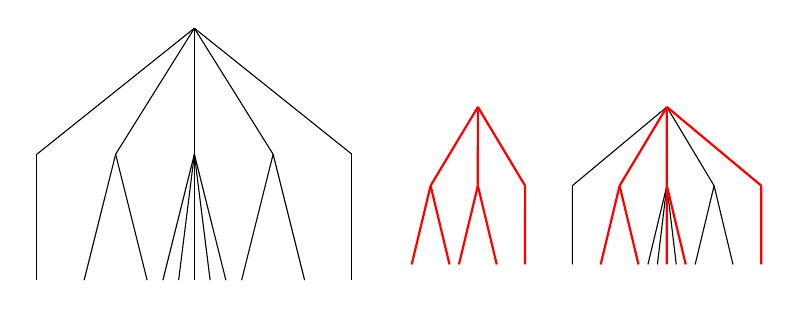
\begin{tikzpicture}
  \begin{scope}[xscale=1,yscale=1.6]
  \path (0,0) node[coordinate] (root) {};
  \foreach \x in {-2,...,2}
    {\draw (root) -- (\x,-1) node[coordinate] (n\x) {};}
  \foreach \s/\x/\n in {-2/-2/,
    -1/-1.4/,-1/-.6/,
    0/-.4/,0/-.2/,0/0/,0/.2/,0/.4/,
    1/.6/,1/1.4/,
    2/2/}
    {\draw (n\s) -- (\x,-2) node[below] {$\n$};}
  \end{scope}

  \begin{scope}[xscale=.6,yscale=1]
  \path (6,-1) node[coordinate] (root) {};
  \foreach \x in {-1,0,1}
    {\draw[red, thick] (root) -- (6+\x,-2) node[coordinate] (m\x) {};}
  \foreach \s/\x in {-1/-1.4,
				    -1/-.6,
				    0/-.4,
				    0/.4,
				    1/1}
    {\draw[red, thick] (m\s) -- (6+\x,-3);}

  \path (10,-1) node[coordinate] (root) {};
  \foreach \x in {-2,1}
    {\draw (root) -- (10+\x,-2) node[coordinate] (o\x) {};}
  \foreach \x in {-1,0,2}
    {\draw[red, thick] (root) -- (10+\x,-2) node[coordinate] (o\x) {};}
  \foreach \s/\x in {-2/-2,
			    0/-.4,
			    0/-.2,
			    0/.2,
			    1/.6,
			    1/1.4}
    {\draw (o\s) -- (10+\x,-3);}
  \foreach \s/\x in {-1/-1.4,
    			-1/-.6,
			    0/0,
			    0/.4,
			    2/2}
    {\draw[red, thick] (o\s) -- (10+\x,-3);}
  \end{scope}
\end{tikzpicture}
\caption{On the left, a tree for $d = 4$, which is the smallest $(5,2)$-universal tree:
it has size $11$ (meaning it has $11$ branches).
On the right, a tree of size $5$ and one possible embedding into the universal tree.}
\label{3-fig:example_universal}
\end{figure*}

We say that a tree $t$ embeds into another tree $T$ if:
\begin{itemize}
	\item either both are leaves,
	\item or let $t = [t_1,\dots,t_k]$ and $T = [T_1,\dots,T_{k'}]$, 
	there exist $i_1 < \dots < i_k$ such that for all $j \in [1,k]$ we have that $t_j$ embeds into $T_{i_j}$.
\end{itemize}

\begin{definition}
A tree is $(n,h)$-\textit{universal} if it embeds all trees of size $n$ and height $h$.
\end{definition}

We refer to \cref{3-fig:example_universal} for an example of a $(5,2)$-universal tree.
A first example of an $(n,h)$-universal tree is the tree where each node has degree $n$:
formally we define it recursively by $T_{n,0}$ is a leaf, and $T_{n,h+1} = [\underbrace{T_{n,h},\dots,T_{n,h}}_{n \text{ copies}}]$.
It has size $n^h$.

\subsubsection*{A quasipolynomial universal tree}
We present an inductive construction of a quasipolynomial universal tree.

\begin{theorem}
\label{3-thm:universal_tree}
There exists an $(n,h)$-universal tree with size $f(n,h)$, where $\mu$ satisfies the following:
$$\begin{array}{lll}
f(n,h) & = & f(n,h-1) + f(\lfloor n/2 \rfloor,h) + f(\lceil n/2 \rceil - 1,h), \\
f(n,1) & = & n, \\
f(1,h) & = & 1.
\end{array}$$
%Furthermore, all $(n,h)$-universal trees have size at least $g(n,h)$,
%where $\frac{f(n,h)}{g(n,h)} = O(nh)$.
\end{theorem}
An upper bound is given by
\[
f(n,h) \le 2n \binom{\lceil \log(n) \rceil + h - 1}{\lceil \log(n) \rceil}.
\]
A generous upper bound on the expression above is $n^{O(\log(h))}$.
A refined analysis reveals that the expression is polynomial in $n$ and $h$ if $h = O(\log(n))$.

%We do not prove the lower bound in this chapter.

\begin{proof}
To construct the $(n,h)$-universal tree $T$, let:
\begin{itemize}
	\item $T_\text{left}$ be a $(\lfloor n/2 \rfloor,h)$-universal tree,
	\item $T_\text{middle}$ be a $(n,h-1)$-universal tree,
	\item $T_\text{right}$ be a $(\lceil n/2 \rceil - 1,h)$-universal tree.
\end{itemize}
The intuitive construction of $T$ is as follows: 
we merge the roots of $T_\text{left}$ and $T_\text{right}$ and insert inbetween them
a child of the root to which is attached $T_\text{middle}$.
Formally, let $T_\text{left} = [T^1_{\text{left}},\dots,T^k_{\text{left}}]$ and 
$T_\text{right} = [T^1_{\text{right}},\dots,T^{k'}_{\text{right}}]$,
we define $T$ as
\[
[T^1_{\text{left}},\dots,T^k_{\text{left}},\ T_\text{middle},\ T^1_{\text{right}},\dots,T^{k'}_{\text{right}}].
\]
The construction is illustrated in \cref{3-fig:smallest_tree_construction}.

\begin{figure}[!ht]
\centering
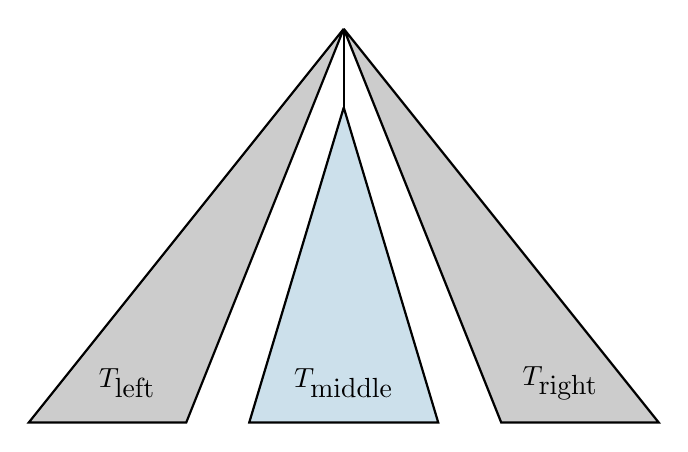
\begin{tikzpicture}
  \begin{scope}[line width=.8pt]
  \foreach \sign/\dir in {-/left,/right}
    {\draw[fill=black!20!white] (0,0) -- (\sign 4,-5) -- (\sign 2,-5) -- (0,0);
     \path (\sign 2.75,-4.5) node {$T_{\textup{\dir}}$};}
  \draw[fill=blue!60!green!20!white] (0,-1) -- (-1.2,-5) -- (1.2,-5) -- (0,-1);
  \path (0,-4.5) node {$T_{\textup{middle}}$};
  \draw (0,0) -- (0,-1);
  \end{scope}
\end{tikzpicture}
\caption{The inductive construction.}
\label{3-fig:smallest_tree_construction}
\end{figure}

\vskip1em
We argue that $T$ is $(n,h)$-universal.
Consider a tree $t = [t_1,\dots,t_k]$ with $n$ branches.
The question is where to cut, \textit{i.e.} which subtree of $t$ gets mapped to $T_\text{middle}$.
Let $n(t_i)$ be the number of branches in $t_i$. 
Since $t$ has $n$ branches, we have $n(t_1) + \cdots + n(t_k) = n$.
There exists a unique $p \in [1,k]$ such that 
$n(t_1) + \cdots + n(t_{p-1}) \le \lfloor n/2 \rfloor
\text{ and } 
n(t_1) + \cdots + n(t_p) > \lfloor n/2 \rfloor$.
The choice of $p$ implies that $n(t_{p+1}) + \cdots + n(t_k) \le \lceil n/2 \rceil - 1$.
To embed $t$ into $T$, we proceed as follows:
\begin{itemize}
	\item the tree $[t_1,\dots,t_{p-1}]$ has at most $\lfloor n/2 \rfloor$ branches,
	so it embeds into $T_\text{left}$ by induction hypothesis;
	\item the tree $t_p$ has height $h-1$ and at most $n$ branches, so in embeds into $T_\text{middle}$ by induction hypothesis;
	\item the tree $[t_{p+1},\dots,t_k]$ has at most $\lceil n/2 \rceil - 1$ branches,
	so it embeds into $T_\text{right}$ by induction hypothesis.
\end{itemize}
\end{proof}
\noindent The construction given in the proof yields the smallest $(5,2)$-universal tree illustrated in \Cref{3-fig:example_universal}.

\subsubsection*{Ordering the branches}
Let us consider a tree $t$.
A branch is given by a list of directions that we define now.
For technical convenience that will manifest itself later, the list of directions is indexed by odd numbers $p \in [1,d]$ downwards:
for example for $d = 10$ a branch is $(D_9,D_7,D_5,D_3,D_1)$.
We often naturally identify a leaf, its branch, and the list of directions that represents it.

We write $B_t$ for the set of branches of $t$ and $\le$ for the lexicographic order on $B_t$.
Note that its interpretation on the tree is: for two branches $b,b'$, we have $b \le b'$ if and only if $b$ is to the left of $b'$.
The strict version of $\le$ is $<$.

We introduce a set of relations $\vartriangleleft_p$ over $B_t$ for each $p \in [1,d]$.
For a branch $b = (D_{d-1},\dots,D_3,D_1)$ we write $b_{\ge p}$ for the tuple $(D_{d-1},\dots,D_{p+2},D_p)$,
which we call the $p$-truncated branch of $b$.
\begin{itemize}
	\item For $p$ odd, we say that $b \vartriangleleft_p b'$ 
	if $b_{\ge p}\ <\ b'_{\ge p}$.
	\item For $p$ even, we say that $b \vartriangleleft_p b'$ 
	if $b_{\ge p}\ \le\ b'_{\ge p}$.
\end{itemize}

To interpret $\vartriangleleft_p$ on the tree, we label the levels by priorities from bottom to top as in \Cref{3-fig:example_universal}.
Then $b \vartriangleleft_p b'$ if and only if the $p$-truncated branch of $b$ is to the left of the $p$-truncated branch of $b'$,
strictly if $p$ is odd, and non-strictly if $p$ is even.

\begin{figure*}[!ht]
\centering
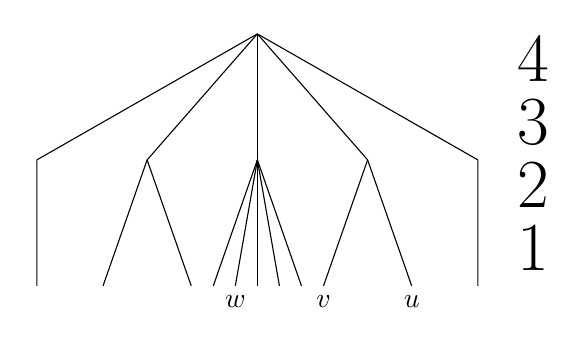
\begin{tikzpicture}
  \begin{scope}[xscale=1.4,yscale=1.6]
  \path (0,0) node[coordinate] (root) {};
  \foreach \x in {-2,...,2}
    {\draw (root) -- (\x,-1) node[coordinate] (n\x) {};}
  \foreach \s/\x/\n in {-2/-2/,
    -1/-1.4/,-1/-.6/,
    0/-.4/,0/-.2/w,0/0/,0/.2/,0/.4/,
    1/.6/v,1/1.4/u,
    2/2/}
    {\draw (n\s) -- (\x,-2) node[below] {$\n$};}
  \foreach \y/\l in {0.2/4,.7/3,1.2/2,1.7/1}
    {\draw (2.5,-\y) node {\begin{Huge}\l\end{Huge}};}
  \end{scope}
\end{tikzpicture}
\caption{Illustration of the relations $\vartriangleleft_p$.}
\label{3-fig:example_relations}
\end{figure*}

We refer to \cref{3-fig:example_relations} for some examples:
\[
v \vartriangleleft_1 u \quad ; \quad  
v \vartriangleleft_2 u \quad ; \quad 
u \vartriangleleft_2 v \quad ; \quad 
w \vartriangleleft_3 u \quad ; \quad 
w \vartriangleleft_2 v.
\]

\begin{lemma}
\label{3-lem:properties_tree}
The relations $\vartriangleleft_p$ for $p \in [1,d]$ induced by a tree $t$ satisfy the following properties:
\begin{itemize}
	\item $\vartriangleleft_d$ is the full relation: for all $b,b'$ we have $b \vartriangleleft_d b'$;
	\item if $b \vartriangleleft_p b'$ and $b' \vartriangleleft_q b''$ then $b \vartriangleleft_{\max(p,q)} b''$;
	\item the relation $\vartriangleleft_p$ is non-reflexive if $p$ is odd;
	\item the relation $\vartriangleleft_1$ is total;
	\item for $p < d$ even we have $b \vartriangleleft_p b'$ if and only if $\neg (b' \vartriangleleft_{p+1} b)$.
\end{itemize}
%Conversely, for any set of relations $\vartriangleleft_p$ for $p \in [1,d]$ over some set $V$ of size $n$ satisfying the properties above,
%there exists a tree $t$ using $V$ as set of leaves inducing these relations.
\end{lemma}
%\begin{proof}
%It is clear that the relations $\vartriangleleft_p$ induced by a tree satisfy the properties.
%
%Conversely, we give an inductive construction.
%Let us assume that the relations $\vartriangleleft_p$ are over the set $V$ of size $n$.
%At any given point we are considering a subset $S$ of $V$ and an odd priority $p$, 
%initially the whole set $V$ and the priority $d-1$.
%Given $S$ and $p$, we partition $S$ as follows:
%$S_1$ is the set of minimal elements from $S$ with respect to $\vartriangleleft_p$, 
%then $S_2$ the set of minimal elements from $S \setminus S_1$ with respect to $\vartriangleleft_p$,
%and so on: $S_k$ is the set of minimal elements from $S \setminus \bigcup_{j < k} S_j$ with respect to $\vartriangleleft_p$.
%We inductively construct the trees associated to each $S_i$ and $p-2$, yielding the tree for $S$ and $p$.
%The fact that the relation $\vartriangleleft_1$ is total implies that the leaves of the tree we construct correspond to singletons of $V$,
%hence can be identified with $V$.
%\end{proof}

The following observation rephrases the notion of embeddings between trees using the ordering on branches.

\begin{fact}
\label{3-fact:embedding}
Let $t,T$ be two trees.
Then $t$ embeds into $T$ if and only if there exists a function $\mu : B_t \to B_T$
such that for all branches $b,b'$:
\[
b \vartriangleleft_p^t b' \implies \mu(b) \vartriangleleft_p^T \mu(b').
\]
\end{fact}

\subsubsection*{Progress measures}
We explain how a tree $t$ induces both a lattice $(Y_t,\le)$ and a monotonic function $\delta_t : Y_t \times [1,d] \to Y_t$.
The set $Y_t$ is the set of branches of $t$ augmented with a new element $\bot$, 
and $\le$ is the lexicographic order on branches with $\bot$ as least element.
For each $p \in [1,d]$ and $b \in Y_t$ we extend $\vartriangleleft_p$ with $\bot \vartriangleleft_p b$.
We then define $\delta : Y_t \times [1,d] \to Y_t$ by
\[
\delta(b,p) = \max \set{b' : b' \vartriangleleft_p b}.
\]
This in turn induces a monotonic operator $\Op_t : F_V \to F_V$ defined by:
\[
\Op(\mu)(v) = 
\begin{cases}
\max \set{\delta( \mu(v'), \col(v)) : (v,v') \in E} & \text{ if } v \in \VE, \\
\min \set{\delta( \mu(v'), \col(v)) : (v,v') \in E} & \text{ if } v \in \VA.
\end{cases}
\]

Let $\Game$ be a parity game, a progress measure is a function $\mu : V \to Y_t$ which is a post-fixed point: $\mu \le \Op_t(\mu)$. 
Expanding the definitions, this means that for all vertices $v$, we have
\[
\begin{array}{llll}
\exists (v,v') \in E,\ & \mu(v) \le \delta_t( \mu(v'), \col(v)) & \text{ if } v \in \VE, \\
\forall (v,v') \in E,\ & \mu(v) \le \delta_t( \mu(v'), \col(v)) & \text{ if } v \in \VA.
\end{array}
\]
The definition of $\delta_t$ further simplifies it to: for all vertices $v$, we have
\[
\begin{array}{llll}
\exists (v,v') \in E,\ & \mu(v) \vartriangleleft_{\col(v)} \mu(v') & \text{ if } v \in \VE, \\
\forall (v,v') \in E,\ & \mu(v) \vartriangleleft_{\col(v)} \mu(v') & \text{ if } v \in \VA.
\end{array}
\]

The following theorem is our first and main step towards proving the characterisation principle.

\begin{theorem}
\label{3-thm:progress_measure}
Let $\Game$ be a parity game and $v$ a vertex.
Then Eve wins from $v$ if and only if there exists a tree $t$ and a progress measure $\mu : V \to Y_t$ such that $\mu(v) \neq \bot$.
\end{theorem}

In order to prove \cref{3-thm:progress_measure}, we first consider the case of parity graphs.
A progress measure in a parity graph is a function $\mu : V \to Y_t$ such that 
for all edges $(v,v') \in E$ we have $\mu(v) \vartriangleleft_{\col(v)} \mu(v')$.

Recall that a graph satisfies parity from $v$ if all infinite paths from $v$ satisfy parity.
This is equivalent to asking whether all cycles reachable from $v$ are even, meaning the maximal priority appearing in the cycle is even.

\begin{lemma}
\label{3-lem:progress_measure}
Let $G$ be a parity graph and $v$ a vertex.
Then $G$ satisfies parity from $v$ if and only if 
there exists a tree $t$ and a progress measure $\mu : V \to Y_t$ such that $\mu(v) \neq \bot$.
\end{lemma}

\begin{proof}
Let us assume that there exists a tree $t$ and a progress measure $\mu : V \to Y_t$ such that $\mu(v) \neq \bot$
and for all edges $(v,v') \in E$ we have $\mu(v) \vartriangleleft_{\col(v)} \mu(v')$.
To show that $G$ satisfies parity from $v$ we show that any cycle reachable from $v$ is even.
Let us consider such a cycle:
\[
(v_1,v_2) (v_2,v_3) \cdots (v_k,v_1).
\]
Since the cycle is reachable from $v$ and $\mu(v) \neq \bot$, this implies that $\mu(v_i) \neq \bot$ for $i \in [1,k]$.
Let us assume towards contradiction that its maximal priority is odd, and without loss of generality it is $\col(v_1)$.
Applying our hypothesis to each edge of the cycle we have
\[
\mu(v_1) \vartriangleleft_{\col(v_1)} \mu(v_2) \vartriangleleft_{\col(v_2)} \cdots 
\vartriangleleft_{\col(v_{k-1})} \mu(v_k) \vartriangleleft_{\col(v_k)} \mu(v_1).
\]
The second item of \cref{3-lem:properties_tree} implies that $\mu(v_1) \vartriangleleft_{\col(v_1)} \mu(v_1)$, 
which contradicts the third item since $\vartriangleleft_{\col(v_1)}$ is non-reflexive given that $\col(v_1)$ is odd.

\vskip1em
Let us now prove the converse implication.
We prove the following property by induction on the number of vertices:
for all graphs satisfying parity (without the usual assumption that every vertex has an outgoing edge),
there exists a tree $t$ and a progress measure $\mu : V \to Y_t$ such that $\mu(v) \neq \bot$
for all vertices~$v \in V$.

There are two cases: either the largest priority $d$ in the graph is even or it is odd.
We write $V_d$ for the set of vertices of priority $d$. 

\vskip1em
\textit{Case $d$ even.}
Let us consider the graph induced by the set of vertices $V \setminus V_d$.
It satisfies parity, so by induction hypothesis there exists a tree $t$ and a progress measure $\mu_d : V \setminus V_d \to Y_t$ 
such that $\mu_d(v) \neq \bot$ for all vertices $v \in V \setminus V_d$.
We extend $\mu_d$ to $\mu : V \to Y_t$: for $v \in V_d$ we let $\mu(v) = \ell_{\max}$ where $\ell_{\max}$ is the maximal element in $Y_t$.
Then $\mu$ is a progress measure such that $\mu_d(v) \neq \bot$ for all vertices $v \in V$.
Indeed the additional edges are of the form $(v,v')$ for either $v \in V_d$ or $v' \in V_d$:
in the first case $\mu(v) \vartriangleleft_{\col(v)} \mu(v')$ holds because $\vartriangleleft_d$ is the full relation,
and in the second case because $\mu(v') = \ell_{\max}$.

\vskip1em
\textit{Case $d$ odd.}
We claim that there exists a non-trivial partition $V = W_1 \uplus W_2$ such that there is no edge from $W_1$ to $W_2$.
Let $u \in V_d$, define $U$ the set of vertices reachable from $u$ by a non-trivial path.
If $U$ is empty, then $V = \set{u} \uplus (V \setminus \set{u})$ is a non-trivial partition as desired.
Otherwise $U$ is non empty, then $V = U \uplus (V \setminus U)$ is a non-trivial partition as desired:
to see that $V \setminus U$ is non empty we note that $u \in V \setminus U$, otherwise there would be an odd cycle 
(containing the maximal and odd priority $d$).

We consider the graphs induced by $W_1$ and $W_2$.
They both satisfy parity, so by induction hypothesis for $i \in \set{1,2}$ 
there exists a tree $t_i$ and a progress measure $\mu_i : W_i \to Y_{t_i}$ 
such that $\mu_i(v) \neq \bot$ for all vertices $v \in W_i$.
We let $t$ denote the tree obtained by putting the two trees $t_1$ and $t_2$ side by side with $t_2$ on the left of $t_1$.
Formally, $t_1 = [t^1_1,\dots,t^k_1]$ and $t_2 = [t^1_2,\dots,t^{k'}_2]$, let 
$t = [t^1_2,\dots,t^{k'}_2,\ t^1_1,\dots,t^k_1]$.
We define $\mu : V \to Y_t$ by $\mu(v) = \mu_i(v)$ if $v \in W_i$.
Then $\mu$ is a progress measure: for edges in the graphs induced by $W_1$ and $W_2$ this is because $\mu_1$ and $\mu_2$ are,
and the additional edges are from $v \in W_2$ to $v' \in W_1$, so indeed $\mu(v) \vartriangleleft_{\col(v)} \mu(v')$ holds.
This finishes the inductive proof of the property.

\vskip1em
We show that the property extends to graphs not satisfying parity.
Let $G$ a parity graph and $W$ the set of vertices $v$ such that $G$ satisfies parity from $v$.
Let $G'$ the graph induced by $W$, it satisfies parity so 
by the property above there exists a tree $t$ and a progress measure $\mu_W : W \to Y_t$ such that
$\mu_W(v) \neq \bot$ for all vertices $v \in W$.
We extend $\mu_W$ to $\mu : V \to Y_t$: for $v \notin W$ we let $\mu(v) = \bot$.
To see that $\mu$ is a progress measure we make two remarks.
First, if $v \in W$ then all successors of $v$ are also in $W$ (by prefix independence of parity),
so the edges in $G$ are either in $G'$ or from $v \in V \setminus W$ to $v' \in W$.
In the first case $\mu(v) \vartriangleleft_{\col(v)} \mu(v')$ holds because $\mu_W$ is a progress measure,
and in the second case because $\mu(v) = \bot$.
\end{proof}

We can now prove \cref{3-thm:progress_measure}.

\begin{proof}
Assume that Eve wins from $v$ and let $\sigma$ be a positional strategy.
The parity graph $\Game[\sigma]$ satisfies parity from $v$, so thanks to \cref{3-lem:progress_measure}
there exists a tree $t$ and a function $\mu : V \to Y_t$ such that $\mu(v) \neq \bot$
and for all edges $(v,v') \in E$ we have $\mu(v) \vartriangleleft_{\col(v)} \mu(v')$.
We remark that $\mu : V \to Y_t$ is actually a progress measure: the condition for $v \in \VE$ is ensured by the edge $\sigma(v)$,
and the condition for $v \in \VA$ by assumption on $\mu$.

\vskip1em
Conversely, assume that there exists a tree $t$ and a progress measure $\mu : V \to Y_t$.
It induces a positional strategy defined by $\sigma(v) = (v,v')$ such that $\mu(v) \vartriangleleft_{\col(v)} \mu(v')$.
We argue that $\sigma$ is a winning strategy from any vertex $v$ such that $\mu(v) \neq \bot$.
This is a consequence of \cref{3-lem:progress_measure} for the parity graph $\Game[\sigma]$.
\end{proof}

\Cref{3-thm:progress_measure} is very close to the characterisation principle we are after,
the only difference being that the lattice $(Y_t,\le)$ depends on an existentially quantified tree $t$.
This is where we use universal trees:

\begin{corollary}
\label{3-cor:progress_measure}
Let $\Game$ be a parity game with $n$ vertices and priorities in $[1,d]$, and $v$ a vertex.
Let $T$ be a $(n,d/2)$-universal tree.
Then Eve wins from $v$ if and only if there exists a progress measure $\mu : V \to Y_T$ such that $\mu(v) \neq \bot$.
\end{corollary}

\begin{proof}
Assume that Eve wins from $v$, thanks to \cref{3-thm:progress_measure} there exists a tree $t$ and a progress measure $\mu : V \to Y_t$ 
such that $\mu(v) \neq \bot$.
Since $T$ is $(n,d/2)$-universal and~$t$ has at most $n$ branches, $t$ embeds into $T$,
which thanks to \cref{3-fact:embedding} implies that there exists $\mu' : B_t \to B_T$ respecting the relations $\vartriangleleft$.
We extend it to $\mu' : Y_t \to Y_T$ by $\mu'(\bot) = \bot$.
Then the composition $\mu' \circ \mu : V \to Y_T$ is a progress measure such that $(\mu' \circ \mu)(v) \neq \bot$. 

The converse implication is a direct consequence of \cref{3-thm:progress_measure}.
\end{proof}

We have proved that the characterisation principle holds for any $(n,d/2)$-universal tree.

\subsection*{The algorithm}
Let us fix $T$ an $(n,d/2)$-universal tree.
It induces both a lattice $(Y_T,\le)$ and a monotonic function $\delta_T : Y_T \times [1,d] \to Y_T$,
which in turn induces a monotonic operator $\Op_T : F_V \to F_V$.
Since $T$ is fixed we do not specify the subscript $T$ for all these objects.

%Thanks to \cref{3-cor:progress_measure} the characterisation principle holds:
%Eve wins from $v$ if and only if there exists a progress measure $\mu : V \to Y$ such that $\mu(v) \neq \bot$.

The last step is to construct an algorithm returning the maximal progress measure relying on Kleene's fixed point theorem (stated as \cref{1-thm:kleene}).
The generic algorithm is explained in \cref{1-sec:value_iteration}, let us instantiate it here.

For the complexity analysis it is useful to decompose $\Op$ into a set of operators:
\[
\Op_v(\mu)(u) = 
\begin{cases}
\mu(v) & \text{ if } u \neq v, \\
\max \set{\delta( \mu(v'), \col(v)) : (v,v') \in E} & \text{ if } u = v \in \VE, \\
\min \set{\delta( \mu(v'), \col(v)) : (v,v') \in E} & \text{ if } u = v \in \VA.
\end{cases}
\]

We introduce some terminology: we say that an edge $e = (v,v')$ is \textit{neglected} if $\neg (\mu(v) \vartriangleleft_{\col(v)} \mu(v'))$,
and a vertex $v$ is \textit{neglected} if $\neg (\mu(v) \le \Op_v(\mu)(v))$.

\begin{figure}[!ht]
\centering
\begin{tikzpicture}
  \node[s-adam] (v) at (0,-2) {$\begin{array}{c} v \\ 3 \end{array}$};
  \node[s-eve] (v') at (2,-1) {$v'$};
  \node[s-eve] (v'') at (2,-3) {$v''$};    

    \path[arrow]
      (v) edge (v')
      (v) edge (v'');

  \begin{scope}[xscale=1.4,yscale=1.6]
  \path (5,0) node[coordinate] (root) {};
  \foreach \x in {-2,...,2}
    {\draw (root) -- (5+\x,-1) node[coordinate] (n\x) {};}
  \foreach \s/\x/\n in {-2/-2/,
    -1/-1.4/,-1/-.6/\Op_v(v),
    0/-.4/,0/-.2/,0/0/,0/.2/v'',0/.4/,
    1/.6/v',1/1.4/,
    2/2/v}
    {\draw (n\s) -- (5+\x,-2) node[below] {$\n$};}

  \node (old) at (5+2,-2.25) {};    
  \node (new) at (5-.6,-2.25) {};    
  \path[arrow]
    (old) edge[bend left, red, thick] (new);

  \foreach \y/\l in {0.2/4,.7/3,1.2/2,1.7/1}
    {\draw (7.5,-\y) node {\begin{Huge}\l\end{Huge}};}
  \end{scope}
\end{tikzpicture}
\caption{The operator $\Op_v$ in action: $\Op_v(\mu)(v)$ is the maximal leaf (meaning the rightmost leaf) 
which satisfies $\Op_v(\mu)(v) \vartriangleleft_3 \mu(v')$ and $\Op_v(\mu)(v) \vartriangleleft_3 \mu(v'')$.}
\label{3-fig:lifting}
\end{figure}

The pseudocode for the algorithm is given in \cref{3-algo:value_iteration}, 
where we let $\ell_{\max}$ denote the maximal leaf in $T$.

\begin{algorithm}[ht]
 \KwData{A parity game with $n$ vertices priorities in $[1,d]$ and a $(n,d/2)$-universal tree $T$.}
 \DontPrintSemicolon

\For{$v \in V$}{
$\mu(v) \leftarrow \ell_{\max}$
}
     
\Repeat{$\forall v \in V,\ \mu \le \Op_v(\mu)$}{
Choose $v \in V$ which is neglected

$\mu \leftarrow \min(\mu, \Op_v(\mu))$}

\Return{$\mu$}
\caption{The value iteration algorithm.}
\label{3-algo:value_iteration}
\end{algorithm}

\begin{theorem}
For all $(n, d/2)$-universal tree $T$, for all parity games $\game$ with $n$ vertices and priorities in $[1,d]$,
the value iteration algorithm over the tree $T$ returns the maximal progress measure $\mu$ for $\game$ over $T$.
\end{theorem}

Thanks to \cref{3-cor:progress_measure}, the maximal progress measure yields a solution for parity games:
Eve wins from $v$ if and only if $\mu(v) \neq \bot$.

\subsection*{Complexity analysis}
The number of times the operator $\Op_v$ is used is bounded by the number of leaves of $T$,
which we write $|T|$, implying that the total number of iterations is bounded by~$n \cdot |T|$.
%This bound cannot be much improved: for instance a vertex of priority $1$ with a self loop is evidently losing but the algorithm
%will use $|T|$ times $\Op_v$ to get this information.
To determine the overall complexity we need to discuss two aspects of the algorithm:
\begin{itemize}
	\item the data structure and in particular the choice of the vertex $v$ in the loop;
	\item the computation of $\Op_v$ and in particular the encoding of branches of $T$.
\end{itemize}

We note that a vertex $v \in \VE$ is neglected if and only if all its outgoing edges are neglected,
and a vertex $v \in \VA$ is neglected if and only if it has a neglected outgoing edge.
Hence checking whether a vertex $v$ is neglected requires considering all of its outgoing edges $(v,v')$
and checking whether $\mu(v) \vartriangleleft_{\col(v)} \mu(v')$.
Let us write $\Delta$ for the complexity of checking whether $\mu(v) \vartriangleleft_{\col(v)} \mu(v')$.
Hence checking whether $v$ is neglected costs 
$O(|\Ing^{-1}(v)| \cdot \Delta)$, where $|\Ing^{-1}(v)|$ is the number of outgoing edges of $v$.

A naive implementation of \cref{3-algo:value_iteration} would in each repeat loop go through every vertex $v$ 
to check whether it is neglected.
This would incur a linear cost: $\sum_{v \in V} O(|\Ing^{-1}(v)| \cdot \Delta) = O(m \cdot \Delta)$.
Thus the overall complexity would be
\[
O((m \cdot \Delta) \cdot (n \cdot |T|)) = O(nm \cdot \Delta \cdot |T|).
\]
Typically $\Delta$ is small (we will see that for a well chosen universal tree $T$ it is polylogarithmic in $n$ and $d$),
and $T$ is the dominating factor (quasipolynomial in $n$ and $d$ thanks to \cref{3-thm:universal_tree}).

We first explain that using a better data structure we can maintain the list of vertices $v$ such that $\neg (\mu \le \Op_v(\mu))$,
saving a linear factor in the complexity.
We then discuss the cost $\Delta$ by choosing an appropriate encoding of the quasipolynomial universal tree constructed in~\cref{3-thm:universal_tree}.

\subsubsection*{Data structure}
We use a data structure similar to the attractor computation presented in \cref{2-sec:attractors}.
The pseudocode is given in \cref{3-algo:value_iteration_data_structure}.
We did not provide the pseudocode for the functions $\texttt{Init}$ and $\texttt{Update}$.

The data structure consists of the following objects:
\begin{itemize}
	\item a leaf of $T$ for each vertex, representing the current function $\mu : V \to Y$;
	\item a set $S$ of vertices (each vertex appears at most once in $S$, the order in which vertices are stored and retrieved from the set does not matter);
	\item for each vertex of Eve a number of edges.
\end{itemize}
For our complexity analysis we use the unit cost RAM model, see \cref{1-sec:computation} for details.
In the case at hand let us choose for the machine word size $w = \log(m) + \log(d)$, 
so that an edge together with its priority can be stored in one machine word.
The space complexity of this data structure depends on the encoding of $T$, which we will discuss later.

The invariant of the algorithm satisfied before each iteration of the repeat loop is the following:
\begin{itemize}
	\item for $v \in \VA$, the value of $\text{number}$-$\text{neglected}$-$\text{edges}(v)$
	is the number of neglected edges of $v$;
	\item $S$ is the set of neglected vertices.
\end{itemize}
The invariant is satisfied initially thanks to the function $\texttt{Init}$.
Let us assume that we choose and remove $v$ from $S$.
Since we modify only $\mu(v)$ the only potentially neglected vertices are in $S$ (minus $v$) and the incoming edges of $v$;
for the latter each of them is checked and added to $S$ when required.
By monotonicity, neglected vertices remain neglected so all vertices in $S$ (minus $v$) are still neglected.
Hence the invariant is satisfied.

The invariant implies that the algorithm indeed implements~\cref{3-algo:value_iteration} hence returns the maximal progress measure, 
but it also has implications on the complexity.
Indeed one iteration of the repeat loop over some vertex $v$ involves 
\[
O\left( (|\Ing^{-1}(v)| + |\Out^{-1}(v)|) \cdot \Delta \right)
\]
operations,
the first term corresponds to updating $\mu(v)$ and $\text{number}$-$\text{neglected}$-$\text{edges}(v)$,
which requires for each outgoing edge of $v$ to compute $\delta$,
and the second term corresponds to considering all incoming edges of $v$ and treating the neglected ones.
Thus the overall complexity is
\[
O\left( 
\sum_{v \in V} (|\Ing^{-1}(v)| + |\Out^{-1}(v)|) \cdot \Delta \cdot |T|
\right) 
= O(m \cdot \Delta \cdot |T|).
\]

\begin{algorithm}
 \KwData{A parity game with $n$ vertices priorities in $[1,d]$ and a $(n,d/2)$-universal tree $T$.}
 \SetKwFunction{FTreat}{Treat}
 \SetKwFunction{FVI}{ValueIteration}
 \SetKwFunction{FInit}{Initialise}
 \SetKwFunction{FUpdate}{Update}
 \SetKwProg{Fn}{Function}{:}{}
 \DontPrintSemicolon
 
\Fn{\FVI{}}{
%	\For{$v \in V$}{
%		$\mu(v) \leftarrow \ell_{\max}$
%	}
	
	\FInit{$\mu$, $\text{number}$-$\text{neglected}$-$\text{edges}$, $S$}

%	\vskip1em
%	\For{$e \in E$}{	
%		\If{$e$ is neglected}{
%			\FTreat($e$)
%		}
%	}

	\vskip1em
	\Repeat{$S$ empty}{
		Choose some $v$ in $S$ and remove it from $S$

		$\mu \leftarrow \min(\mu, \Op_v(\mu))$

		\FUpdate{$\text{number}$-$\text{neglected}$-$\text{edges}(v)$}

		\For{$e \in E$ \text{ such that } $\Out(e) = v$}{
			\If{$e$ is neglected}{
				\FTreat($e$)
			}
		}
	}

	\Return{$\mu$}
}

\vskip1em
\Fn{\FTreat{$e$}}{
	$v \leftarrow \Ing(e)$
	
	\If{$v \in \VA$ and $v \notin S$}{
		Add $v$ to $S$		
	}
	
	\If{$v \in \VE$ and $v \notin S$}{	
		$\text{number}$-$\text{neglected}$-$\text{edges}(v) \leftarrow \text{number}$-$\text{neglected}$-$\text{edges}(v) + 1$

		\If{$\text{number}$-$\text{neglected}$-$\text{edges}(v) = $ number of outgoing edges of $v$}{
			Add $v$ to $S$
		}
	}
}
\caption{The value iteration algorithm with explicit data structure.}
\label{3-algo:value_iteration_data_structure}
\end{algorithm}

\subsubsection*{Encoding branches}
Let us fix $T$ to be the quasipolynomial universal tree constructed in \cref{3-thm:universal_tree}.

In our definition of trees we say that a tree is an ordered list of subtrees $[t_1,\dots,t_k]$,
so we use $[1,k]$ with the natural order for ordering the subtrees.
Any other total order can be used to that effect, and a more appropriate order may lead to smaller encoding.
Indeed, using $[1,k]$ for ordering subtrees, if a tree has height $h$ and $n$ branches then a branch is a sequence of $h$ numbers in $[1,n]$,
so it uses $O(h \log(n))$ bits.

Let us consider an order well suited for encoding $T$.
We use $\set{0,1}^*$ the set of binary words and order them using the following three rules that apply for any $u,v \in \set{0,1}^*$:
\[
0u < \varepsilon < 1u \quad ; \quad (0u < 0v \Longleftrightarrow u < v) \quad ; \quad (1u < 1v \Longleftrightarrow u < v).
\]
For words of length at most $2$ the order is $00 < 0 < 01 < \varepsilon < 10 < 1 < 11$.

\begin{figure}[!ht]
\centering
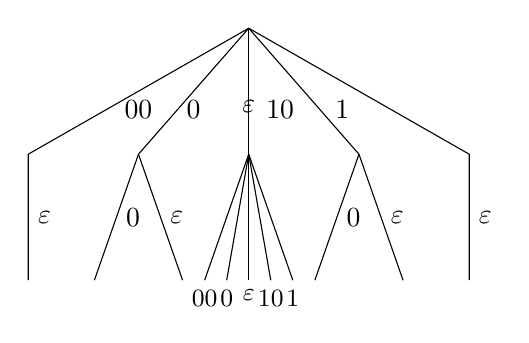
\begin{tikzpicture}
  \begin{scope}[xscale=1.4,yscale=1.6]
  \path (0,0) node[coordinate] (root) {};
  \foreach \x/\n in {-2/00,
  				-1/0,
  				0/\varepsilon}
    {\draw (root) -- node[below] {$\n$} (\x,-1) node[coordinate] (n\x) {};}
  \foreach \x/\n in {1/10,
  				2/1}
    {\draw (root) -- node[below left] {$\n$} (\x,-1) node[coordinate] (n\x) {};}

  \foreach \s/\x/\n in {-2/-2/\varepsilon,
					-1/-1.4/0,
					-1/-.6/\varepsilon,
    				1/.6/0,
    				1/1.4/\varepsilon,
    				2/2/\varepsilon}
    {\draw (n\s) -- node[right] {$\n$} (\x,-2);}
  \foreach \s/\x/\n in {0/-.4/00,
				    0/-.2/0,
				    0/0/\varepsilon,
				    0/.2/10,
				    0/.4/1}
    {\draw (n\s) -- (\x,-2) node[below] {\begin{small}$\n$\end{small}};}
  \end{scope}
\end{tikzpicture}
\caption{The succinct encoding on the $(5,2)$-universal tree.}
\label{3-fig:tree_encoded}
\end{figure}

We can now revisit the construction of the universal tree by defining directly the set of branches.
Recall that $T$ is obtained from $T_\text{left},T_\text{middle}$, and $T_\text{right}$. 
By induction hypothesis branches in $T_\text{left}$ and $T_\text{right}$ are tuples of length $h-1$
and branches in $T_\text{middle}$ tuples of length $h$.
The branches of $T$ are:
\begin{itemize}
	\item branches of $T_\text{left}$ where the first component is prefixed with a $0$;
	\item branches of $T_\text{middle}$ augmented with a new component $\varepsilon$;
	\item branches of $T_\text{right}$ where the first component is prefixed with a $1$.
\end{itemize}
We call this encoding the ""succinct encoding"", it is illustrated in \cref{3-fig:tree_encoded} for the $(5,2)$-universal tree.
The leftmost branch is $(00,\varepsilon)$, and the middle branch $(\varepsilon,\varepsilon)$.
In general, the inductive construction implies that every branch is a tuple $(D_{d-1},\dots,D_1)$ 
such that the sum of the lengths of the directions $D_i$ is at most $\log(n)$.
Thus a branch is encoded using $O(\log(h) \log(n))$ bits: for each of the $\log(n)$ bits we need $\log(h)$ bits to specify its component.

In terms of machine words of size $w = \log(n) + \log(d)$, this means that a branch can be stored using $\log(d)$ machine words.
Hence the data structure uses $O(n \log(d))$ machine words, with together with the input size $O(m)$
means that the space complexity of the algorithm is $O(m + n \log(d))$.

\vskip1em
Using the succinct encoding and a tedious but simple case analysis we can compute $\delta(b,p)$ in time $O(\log(n) \log(d))$.
Putting everything together we obtain the overall complexity 
\[
O\left(nm \log(n) \log(d) \cdot  \binom{\lceil \log(n) \rceil + d/2 - 1}{\lceil \log(n) \rceil} \right),
\]
as stated in \cref{3-thm:value_iteration_quasipoly}.


%%%%%%%%%%%%%%%%%
%%%%%%%%%%%%%%%%%

\section{Strategy improvement algorithms}
\label{1-sec:strategy_improvement}
Value iteration algorithms manipulate value functions and never construct any strategy, at least explicitly.
This is a key difference with strategy improvement algorithms (also called policy iteration algorithms) whose fundamental idea is to maintain and improve a strategy.
We assume that the games we consider in this section are positionally determined, therefore all strategies are assumed to be positional.

\vskip1em
Let us consider a game $\game$ and set as a goal to construct an optimal strategy for Eve.
As for value iteration algorithms we work with a value function: 
the key idea behind strategy improvement is to use $\val^{\sigma}$ to improve the strategy $\sigma$ 
by \emph{switching} an edge, which is an operation that creates a new strategy.
This involves defining the notion of \emph{switchable edge}:
the edge $(v,u)$ is switchable if 
\[
\delta(\val^{\sigma}(u),\col(v)) > \delta(\val^{\sigma}(v'),\col(v)) \text{ where } \sigma(v) = (v,v').
\]
Intuitively: according to $\val^{\sigma}$, playing $(v,u)$ is better than playing $\sigma(v)$.

Given a strategy $\sigma$ and an edge $e = (v,u)$ we use $\sigma[v \to e]$ to denote the strategy playing $e$ from $v$ and all other vertices follow $\sigma$.
Let us write $\sigma \le \sigma'$ if for all vertices $v$ we have $\val^{\sigma}(v) \le \val^{\sigma'}(v)$,
and $\sigma < \sigma'$ if additionally $\neg (\sigma' \le \sigma)$.

The difficulty is that $e = (v,u)$ being switchable does not mean that it is a better move than $\sigma(v)$ in any context,
but only according to the value function $\val^{\sigma}$, so it is not clear that $\sigma[v \to e]$ is better than $\sigma$.
Strategy improvement algorithms depend on the following two principles.

\begin{property}[Progress]
\label{1-property:progress}
Let $\sigma$ be a strategy and let $e = (v,u)$ be a switchable edge. 
Then $\sigma < \sigma[v \to e]$.
\end{property}

\begin{property}[Optimality]
\label{1-property:optimality}
Let $\sigma$ be a strategy that has no switchable edges, then $\sigma$ is optimal.
\end{property}

The algorithm is the following: start at an initial strategy $\sigma_0$. 
In each round $i$ compute $\val^{\sigma_i}$ and look for a switchable edge.
If there exists a switchable edge $e_i = (v_i,v'_i)$, let $\sigma_{i+1} = \sigma_i[v_i \to e_i]$ and iterate to the next round.
Otherwise, return the optimal strategy $\sigma_i$.

The algorithm computes a sequence of strategies 
$\sigma_0 < \sigma_1 < \sigma_2 < \dots$.
Note that any such sequence must be finite, since at each step we strictly increase in the ordering and there are only finitely many (positional) strategies. 

\vskip1em
If both progress and optimality principles hold as stated this yields a strategy improvement algorithm computing the optimal strategy.
Unfortunately such ideal properties rarely hold and it is often necessary to state and prove weaker properties,
we refer to \cref{3-chap:parity,4-chap:payoffs} for examples.
%Let us illustrate this by looking at \cref{1-fig:counter_example_strategy_improvement} representing a CoB{\"u}chi game.
%Assume that the initial strategy is $\sigma_0$ defined by 
%$\sigma_0(v_0) = (v_0,v_1),
%\sigma_0(v_1) = (v_1,v_1)$,
%and $\sigma_0(v_2) = (v_2,v_1)$.
%This strategy is losing from all vertices since it eventually ends up looping around $v_1$.
%This implies that there are no switchable edges and in particular the two winning self loops around $v_0$ and $v_1$ are not considered.
%However $\sigma_0$ is clearly not optimal, contradicting the progress principle.
%
%For this reason the initial strategy $\sigma_0$ must be carefully chosen.
%A solution is to add for each vertex of Eve a new edge for stopping the game, 
%and to define $\sigma_0$ to be the strategy choosing this option from every vertex.
%The benefit of this approach is to avoid declaring some vertices losing only because they are losing with the (badly chosen) initial strategy.
%
%\begin{figure}
%\centering
%  \begin{tikzpicture}[scale=1.3]
%    \node[s-eve] (v0) at (0,0) {$\begin{array}{c} v_0 \\ 2 \end{array}$};
%    \node[s-eve] (v1) at (2,0) {$\begin{array}{c} v_1 \\ 3 \end{array}$};
%    \node[s-eve] (v2) at (4,0) {$\begin{array}{c} v_2 \\ 2 \end{array}$};
%    % create edges
%    \path[arrow]
%      (v1) edge[bend left] (v0)
%      (v0) edge[bend left] (v1)
%      (v1) edge[bend left] (v2)
%      (v1) edge[selfloop=90] (v1)
%      (v2) edge[bend left] (v1)
%      (v2) edge[selfloop=0] (v2)
%      (v0) edge[selfloop=180] (v0);
%  \end{tikzpicture}
%\caption{The optimality principle rarely holds, here illustrated on a CoB{\"u}chi game.}
%\label{1-fig:counter_example_strategy_improvement}
%\end{figure}

\begin{remark}
In the description above we did not specify which switchable edge to choose.
Actually strategy improvement algorithms often switch more than one edge at a time, making this question worse: 
which subset of the switchable edges should be chosen? 
Many possible rules for choosing this set have been studied, as for instance the \emph{greedy all-switches} rule. 
\end{remark}


%%%%%%%%%%%%%%%%%
%%%%%%%%%%%%%%%%%

\section*{Bibliographic references}
\label{1-sec:references}
As discussed in the introduction, the literature on multiobjective models is too vast to provide a full account here. We therefore focus on some directions particularly relevant to our focus.

\paragraph{Multidimension games.} Energy games and their related work were discussed in~\cref{chap:counters}. Our presentation of mean-payoff games is inspired by Velner et al.~\cite{Velner&al:2015}. Brenguier and Raskin studied the Pareto curves of these games in~\cite{Brenguier&Raskin:2015}. While we considered \textit{conjunctions} of mean-payoff objectives, Velner proved that Boolean combinations lead to undecidability~\cite{Velner:2015}.

The undecidability of total-payoff games was first established in~\cite{Chatterjee&al:2015} via reduction from the halting problem for two-counter machines: we provided here a new, simpler proof based on robot games~\cite{Niskanen&Potapov&Reichert:2016}. This undecidability result, along with the complexity barriers of mean-payoff and total-payoff games, motivated the introduction of (multidimension) ""\textit{window objectives}"": conservative variants of mean-payoff and total-payoff objectives that benefit from increased tractability and permit to reason about time bounds~\cite{Chatterjee&al:2015}. Window variants of "parity" objectives have been studied in~\cite{Bruyere&Hautem&Randour:2016}.

\paragraph{Combinations of different objectives.} We focused on multidimension games obtained by conjunction of \textit{identical} objectives. Conjunctions of \textit{heterogeneous} objectives have been studied in a variety of contexts including mean-payoff parity games~\cite{Chatterjee&Henzinger&Jurdzinski:2005,Daviaud&Jurdzinski&Lazic:2018}, energy parity games~\cite{Chatterjee&Doyen:2012,Chatterjee&Randour&Raskin:2014}, average-energy games with energy constraints~\cite{Bouyer&al:2018,Bouyer&al:2017}, simple quantitative objectives~\cite{Bruyere&Hautem&Raskin:2016}. Le Roux, Pauly and Randour studied general conditions under which finite-memory strategies suffice to play optimally, even in a broad multi-objective setting~\cite{LeRoux&Pauly&Randour:2018}.


\paragraph{Beyond worst-case synthesis.} Our presentation is mostly based on~\cite{Bruyere&al:2017}, where all technical details can be found. As noted in~\cite{Bruyere&al:2017}, allowing large inequalities in the BWC problem may require infinite-memory strategies. The case of infinite-memory strategies was studied in~\cite{Clemente&Raskin:2015} along with multidimension BWC mean-payoff problems. BWC problems were studied for other objectives, such as shortest path~\cite{Bruyere&al:2017} or parity~\cite{Berthon&Randour&Raskin:2017}; and on other related models (e.g.,~\cite{Brazdil&Kucera&Novotny:2016,Almagor&Kupferman&Velner:2016}). BWC principles have been implemented in the tool \textsc{Uppaal}~\cite{David&al:2014}.

Comparisons with other rich behavioural models can be found in~\cite{Randour&Raskin&Sankur:2015,Brenguier&al:2016}.

